%% SSC 2026 — CANSSI Postdoc Spotlight
%% Jacob Spertus — 30 minutes, Tuesday 2 June 2026
%%
%% Compile with: latexmk -pdf slides.tex
%% (or upload the ssc-2026/ folder to Overleaf and let it pick main file)
%%
%% Figures live in figures/. Run figures.R to generate the PNGs.
%% Application/empirical plots are placeholders — replace as results land.

\documentclass[10pt,aspectratio=169]{beamer}

% ---------- Theme ----------
\usetheme{metropolis}
\usecolortheme{default}
\metroset{progressbar=frametitle, sectionpage=progressbar, numbering=fraction}

% ---------- Packages ----------
\usepackage{amsmath,amssymb,amsthm,bm}
\usepackage{booktabs}
\usepackage{graphicx}
\usepackage{tikz}
\usepackage{xcolor}
\usepackage{appendixnumberbeamer}
\usepackage{multicol}
\usetikzlibrary{arrows.meta, positioning, calc, decorations.pathreplacing}
\usepackage{natbib}


% If you want citations, uncomment and provide refs.bib:
% \usepackage[backend=biber,style=authoryear,maxcitenames=2]{biblatex}
% \addbibresource{refs.bib}

% ---------- Macros ----------
\newcommand{\E}{\mathbb{E}}
\newcommand{\Prob}{\mathbb{P}}
\newcommand{\R}{\mathbb{R}}
\newcommand{\N}{\mathbb{N}}
\newcommand{\X}{\bm{X}}
\newcommand{\Xt}{\X_{t}}
\newcommand{\Mt}{M_{t}}
\newcommand{\Rt}{R_{t}}
\newcommand{\Lt}{\Lambda_{t}}
\newcommand{\TSM}{\textsc{tsm}}
\newcommand{\SR}{\textsc{s-r}}
\newcommand{\ARL}{\ensuremath{\mathrm{ARL}}}
\newcommand{\PFA}{\ensuremath{\mathrm{PFA}}}
\newcommand{\CAD}{\ensuremath{\mathrm{CAD}}}
\newcommand{\WAD}{\ensuremath{\mathrm{WAD}}}
\newcommand{\Pc}{\mathcal{P}}
\newcommand{\Qc}{\mathcal{Q}}
\newcommand{\Hc}{\mathcal{H}}
\newcommand{\Fc}{\mathcal{F}}
\newcommand{\indep}{\perp\!\!\!\perp}
\newcommand{\bs}{\boldsymbol}

% ---------- Title block ----------
\title{Change-point detection for multiple data streams: betting algorithms and application to infectious disease monitoring}
\subtitle{CANSSI Postdoc Spotlight}
\author{Jacob V.\ Spertus}
\institute{CANSSI postdoc \\ \texttt{jakespertus@gmail.com}}
\date{SSC Annual Meeting --- 2 June 2026}

\begin{document}

% ============================================================
\maketitle
% ============================================================

% ---------- Motivating slide: wastewater up front ----------
\begin{frame}{Motivation: monitoring viral signals in wastewater}
  \begin{columns}[T,onlytextwidth]
    \column{0.55\textwidth}
      \textbf{Problem:} Detect when and where an infectious disease leaves an endemic ``state of control''.
      \medskip

      \textbf{Why it's hard.}
      \begin{itemize}\setlength\itemsep{0.3em}
        \item State of control: what is a meaningful anomaly? 
        \item Noise: catchment areas, sampling protocols, weather, demographics vary in space and time.
        \item Multiplicity: change at different sites at different times.
      \end{itemize}
      \medskip

      \textbf{This talk:} Construct detectors and apply to
      Canadian wastewater data (\textsc{nwmp}).
    \column{0.45\textwidth}
    \centering
    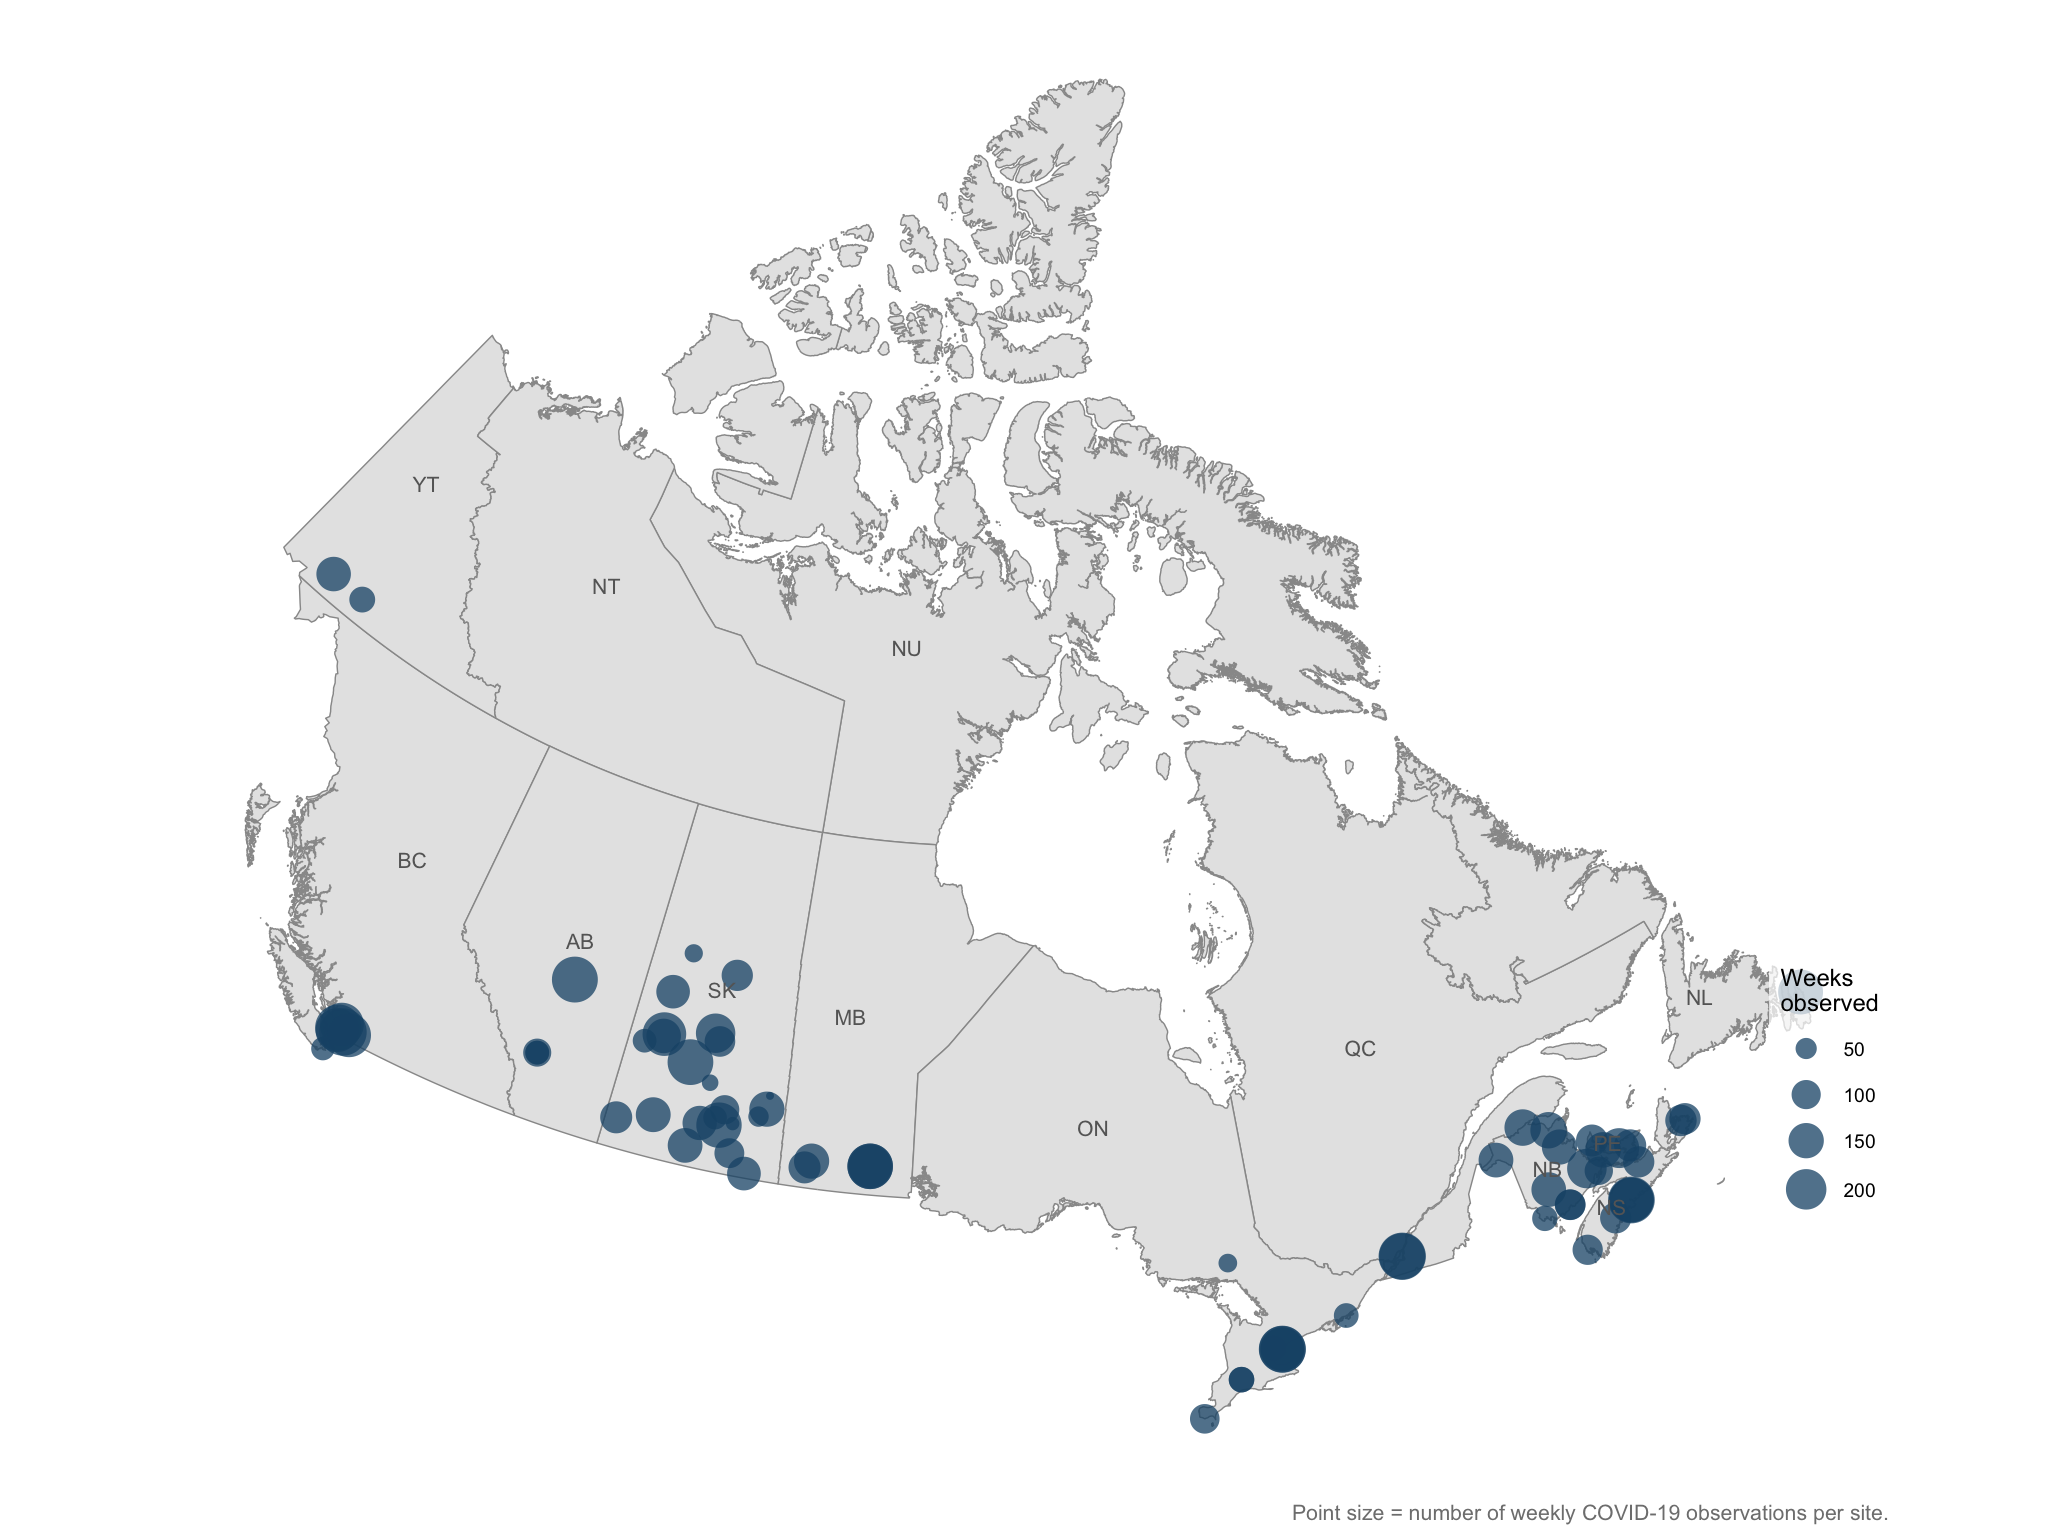
\includegraphics[width=0.8\linewidth]{figures/nwmp_map.png}\\
      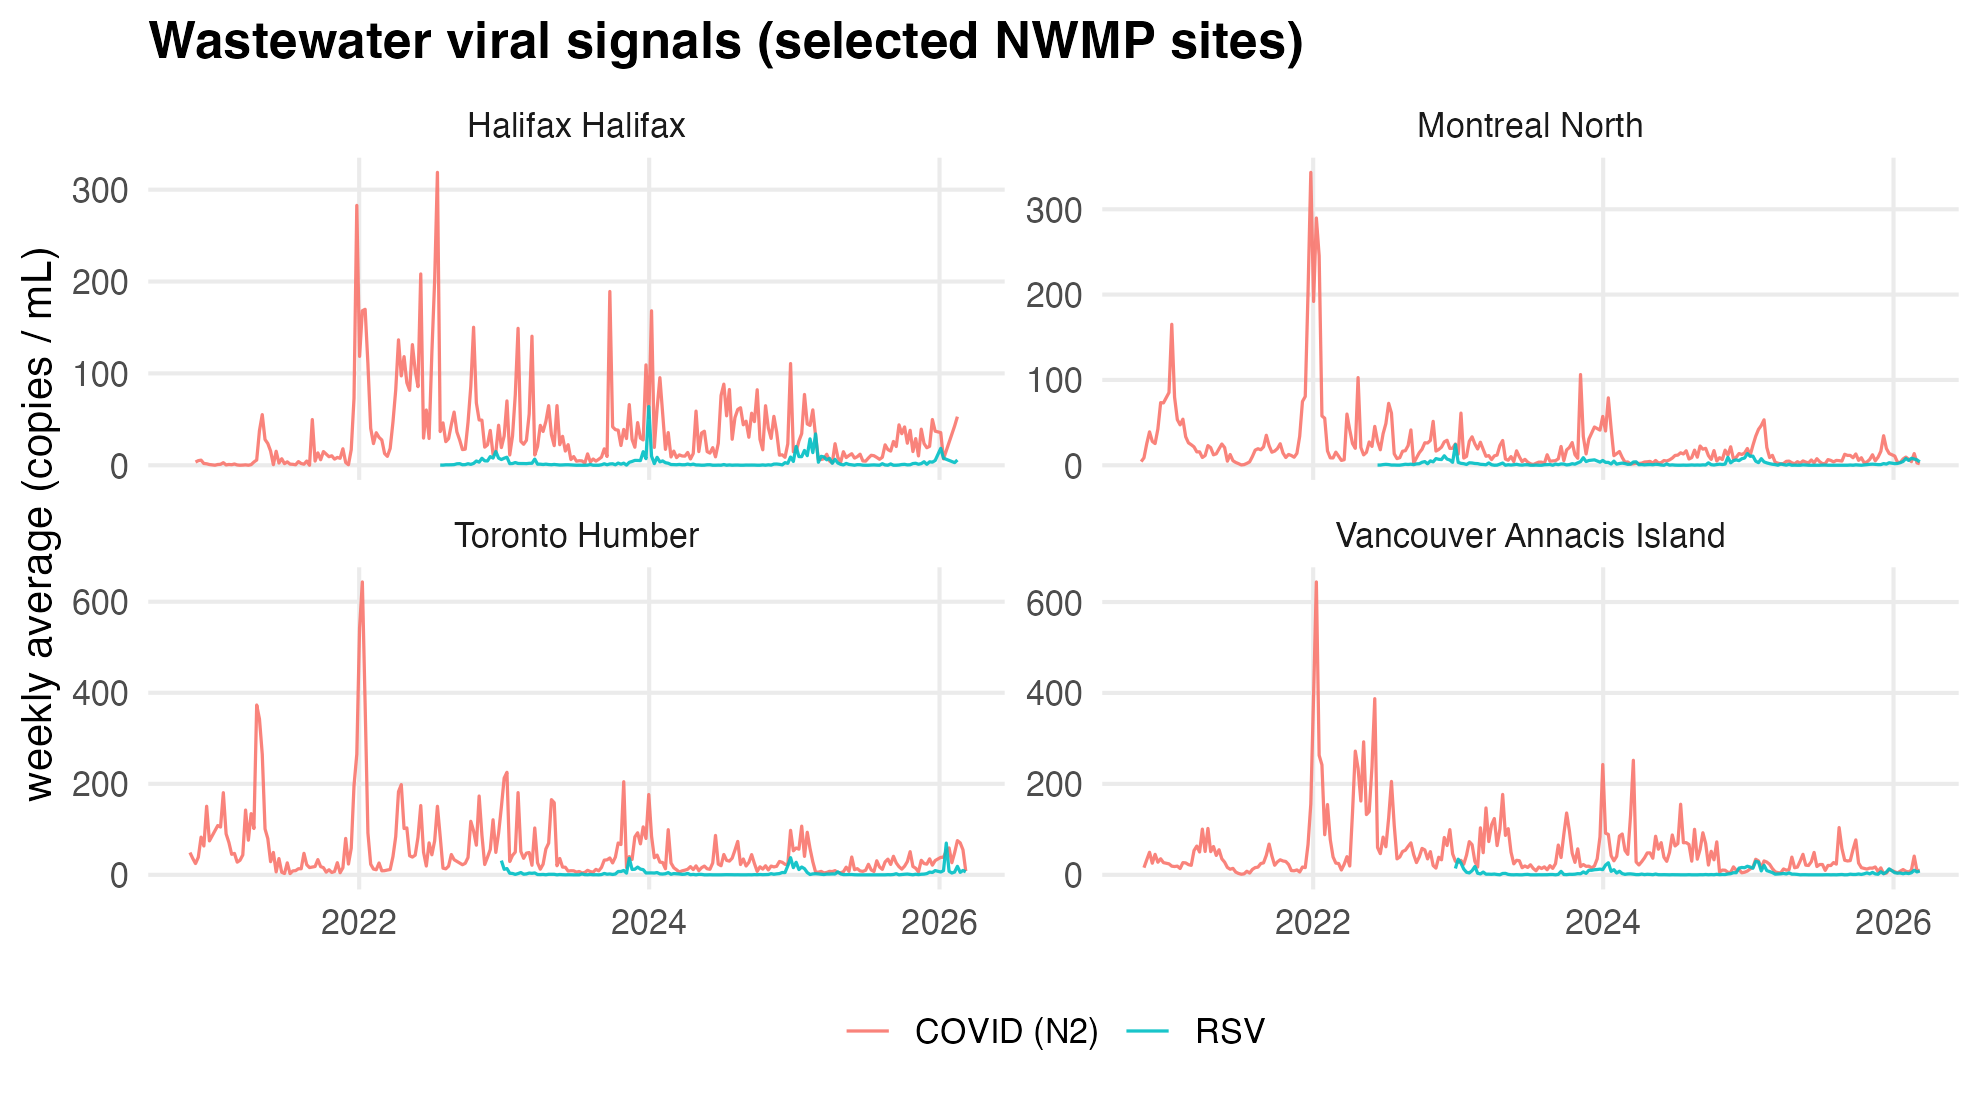
\includegraphics[width=\linewidth]{figures/wastewater_motivation.png}
  \end{columns}
\end{frame}

\begin{frame}{Roadmap}
  \begin{enumerate}\setlength\itemsep{0.6em}
    \item \textbf{Part 1 ($\sim$20 min):} Detection-by-betting
      \begin{itemize}
        \item Goals: validity and efficiency
        \item Martingales, testing-by-betting, and the Shiryaev--Roberts procedure
        \item Joint detectors via combining
        \item Localization via allowances
        \item Simulation snapshot
      \end{itemize}
    \item \textbf{Part 2 ($\sim$10 min):} Wastewater surveillance
  \end{enumerate}
\end{frame}

% ============================================================
\section{Part 1 --- Detection-by-betting}
% ============================================================

% ---------- Change-point setup ----------
\begin{frame}{The sequential multivariate change-point problem}
  Continuously observe a stream of $K$-vectors $(\Xt)_{t \in \N}$ such that:
  \[
    (\Xt)_{t \le \nu} \sim P \in \Pc,\qquad
    (\Xt)_{t > \nu} \sim Q \in \Qc.
  \]
  $\nu \in \N \cup \{\infty\}$ is the unknown \textit{change-point} \\
   \vspace{2mm}
  Full \alert{change-point model} is $(\mathcal{P}, \nu, \mathcal{Q})$ \\
  \vspace{2mm}
  A \alert{detector} $D$ is a stopping time. We want:
  \begin{itemize}
    \item \textbf{Validity:} alarm rate is bounded before change.
    \item \textbf{Efficiency:} short delay after change.
  \end{itemize}
  \medskip
  Conceptual credit: testing-by-betting \citep{ramdasEtal23, grunwaldEtal24} + $E$-detectors \citep{shin_2023}
\end{frame}

\begin{frame}{Example}
      \centering
  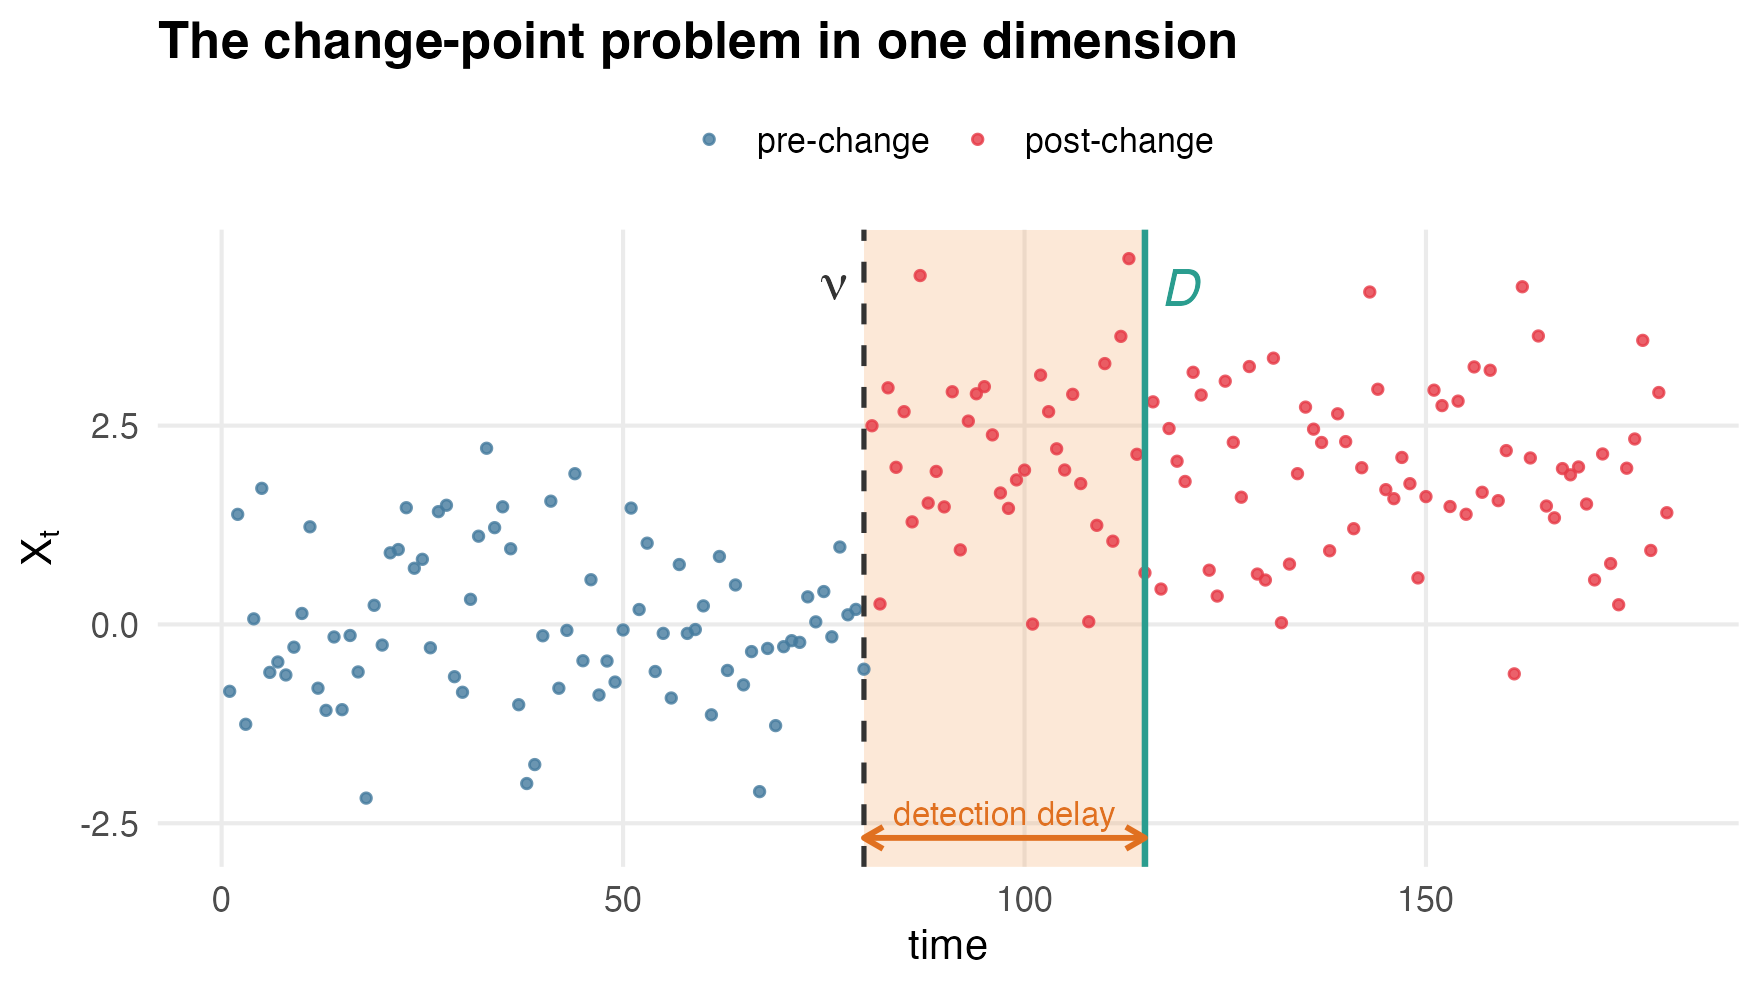
\includegraphics[width=0.95\linewidth]{figures/intro_changepoint.png}
  \vspace{-0.5em}
  \scriptsize 
\end{frame}

\begin{frame}{Some applications}

\begin{itemize}
    \item Industrial product quality \citep{shewart1931}
    \vspace{3mm}
    \item Linear control systems \citep{willsky1976}
     \vspace{3mm}
    \item Online supervised learning \citep{vovk2021}
     \vspace{3mm}
    \item AI for clinical prediction + decision-making \citep{fengEtal2022}
     \vspace{3mm}
    \item Remote health monitoring (BP, EKG, etc.) \citep{kishore2026}
     \vspace{3mm}
    \item Anomalies in sensor and computer networks \citep{shiryaev_1963, xie2013}
     \vspace{3mm}
    \item Structural change in financial models \citep{chu1996, lyu_2024}
\end{itemize}
    % Independence assumption is common, even in nonparametric settings (e.g., \citet{padilla2022, vovk2021})...
\end{frame}

\begin{frame}{Validity: ARL and PFA}

Two error criteria:
\begin{align*}
    \ARL(D) &:= \sup_{P\in\Pc}\E_{P}[D] \\ 
    \PFA(D) &:= \sup_{P\in\Pc}\Prob_{P}(D < \infty)
\end{align*}

  $D$ is \emph{$\ARL$-valid at level $\alpha$} if $\ARL(D) \ge 1/\alpha$\\
  \vspace{3mm}
  $D$ is \emph{$\PFA$-valid} if $\PFA(D) \le \alpha$.\\
\vspace{3mm}
\textbf{This talk:} ARL 
\end{frame}

\begin{frame}{ARL}
    \centering
  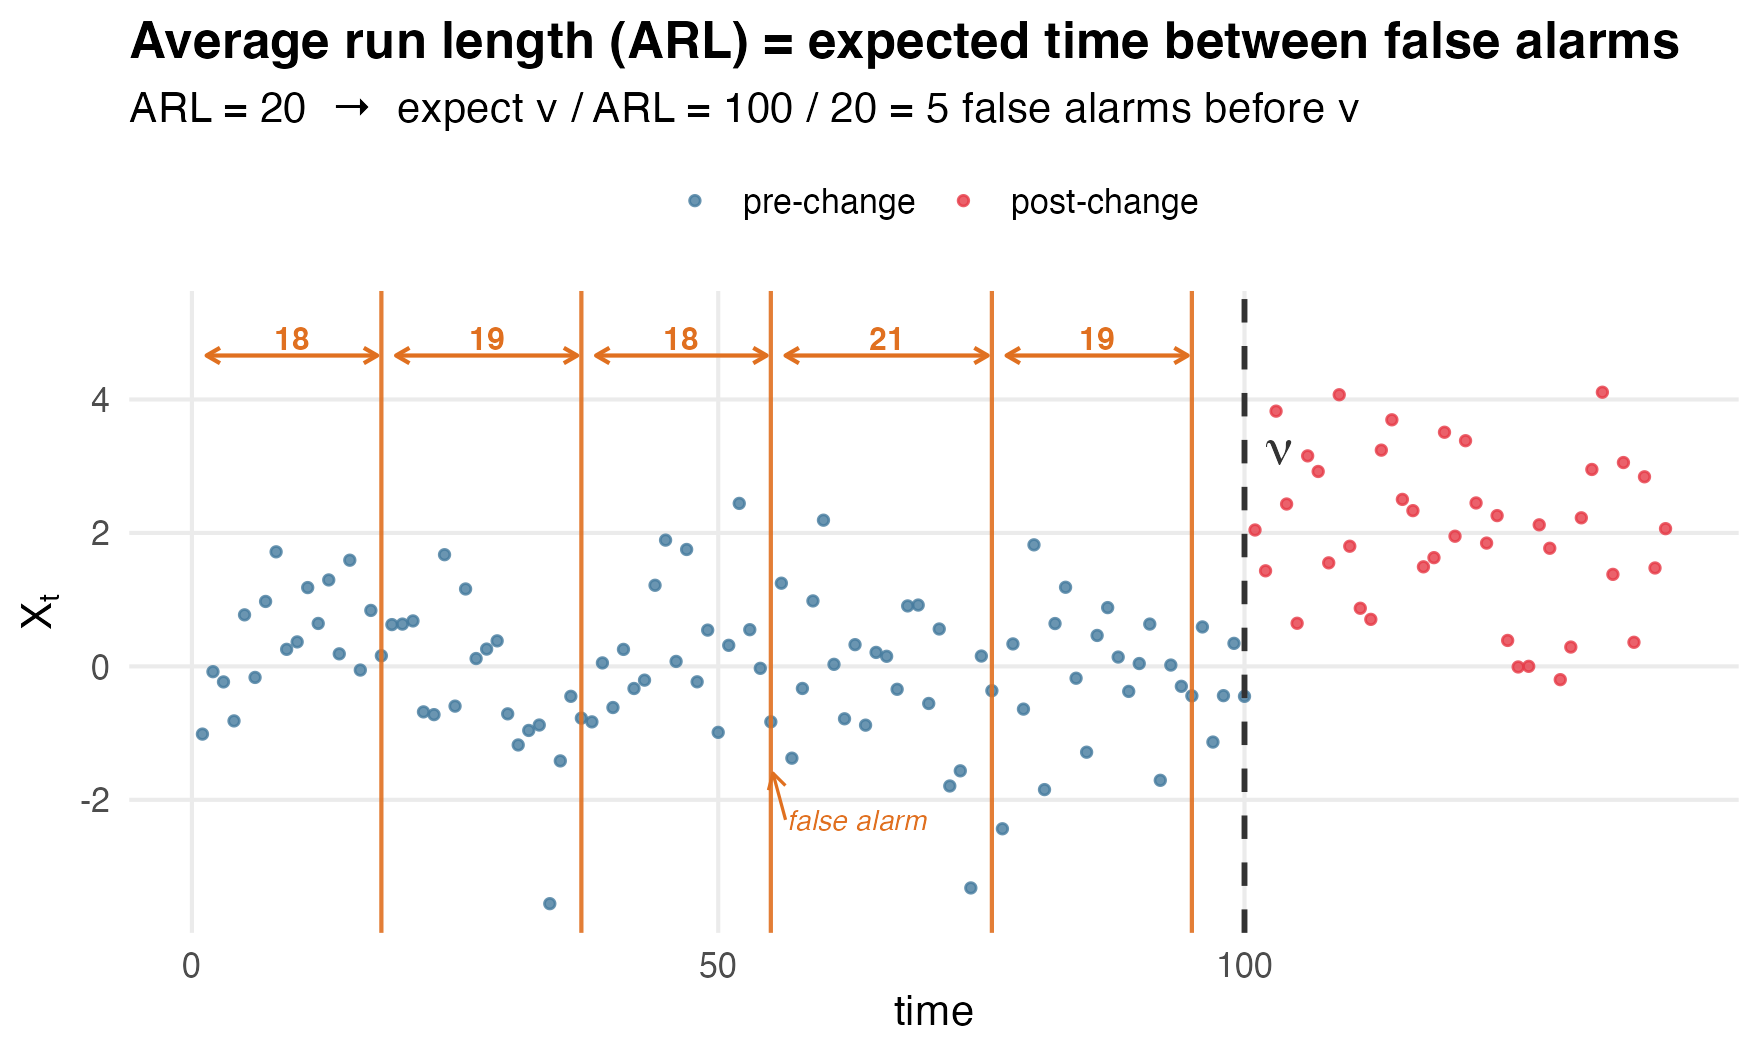
\includegraphics[width=0.95\linewidth]{figures/arl_intuition.png}
  \vspace{-0.5em}
  \scriptsize 
\end{frame}

\begin{frame}{Efficiency}
Conditional average delay:
  $$
\displaystyle
      \CAD(D) := \sup_{\nu\ge 1}\E_{P,\nu,Q}\!\left[(D - \nu) \,\middle|\, D \ge \nu\right]$$
  \begin{itemize}
    \item Averages delay over sample paths where the detector \emph{didn't} already false-alarm.
    \item Define \emph{regret} of $D$ relative to an oracle $D^\star$ that knows $(P,Q)$:
    \[
      \mathrm{regret}(D) := \CAD(D) - \CAD(D^\star).
    \]
    \item An \textit{efficient} detector minimizes regret
  \end{itemize}
  \medskip
  \alert{Goal of this work:} definitely valid, approximately efficient, multivariate detectors.
\end{frame}

% ---------- Test supermartingales: betting ----------
% \begin{frame}{Test supermartingales: a sequential bet against $P$}
% A \textit{filtration} $(\mathcal{F}_t)$ is an expanding sigma-algebra, capturing the information available at time $t$\\ 
% \vspace{2mm}
%   A \alert{test supermartingale} (\TSM) under $\Pc$ is a non-negative process
%   $(\Mt)$ with $M_0 = 1$ and
%   \[
%     \E_P[\Mt \mid \Fc_{t-1}] \le M_{t-1}, \quad \forall~~ P \in \Pc.
%   \]
%   \pause
%   \textbf{Betting interpretation.}
%   Start with \$1. At each round, place a bet against $P$. If $P$ holds,
%   bettor can only \emph{lose money in expectation}. \\
%   \vspace{3mm}
%   Ville's inequality guarantees bettor can probably never make much money:
%   \[
%     \Prob_P\!\left(\exists t : \Mt \ge 1/\alpha\right) \le \alpha.
%   \]
%   \pause
%   \textbf{Concrete \TSM s:}
%   \begin{itemize}
%     \item Likelihood ratio: $\prod_i f_Q(X_i \mid \Hc_i)/f_P(X_i \mid \Hc_i)$.
%     \item Non-negative, mean $\theta$: $\prod_i [1 + \lambda_i (X_i - \theta)]$. 
%   \end{itemize}
%   \textbf{Composite $\Qc$}: predictable estimate $\widehat{Q}$ (quasi-GLR) or mixture over a prior (quasi-Bayesian).
% \end{frame}

% \begin{frame}{Picture: a test supermartingale under no change vs.\ after a change}

% A \textit{test supermartingale} ($M_t$) satisfies $M_0 = 1$ and `does not grow' under $\mathcal{P}$: 
% $$\sup_{P \in \mathcal{P}} \mathbb{E}_P[M_t \mid \mathcal{F}_{t-1}] \leq M_{t-1}$$\\
% \vspace{3mm}
% $M_t$ is probably always small \citep{ville39}: 
% $\sup_{P \in \mathcal{P}} \mathbb{P}_P(\exists~ t: M_t > 1/\alpha) \leq \alpha$\\
% \vspace{3mm}
% % $M_t^{(i)}$ denotes a TSM for $\mathcal{P}$ that starts at time $i$: denote $M_{t-1}^t = 1$
%   \begin{center}
%        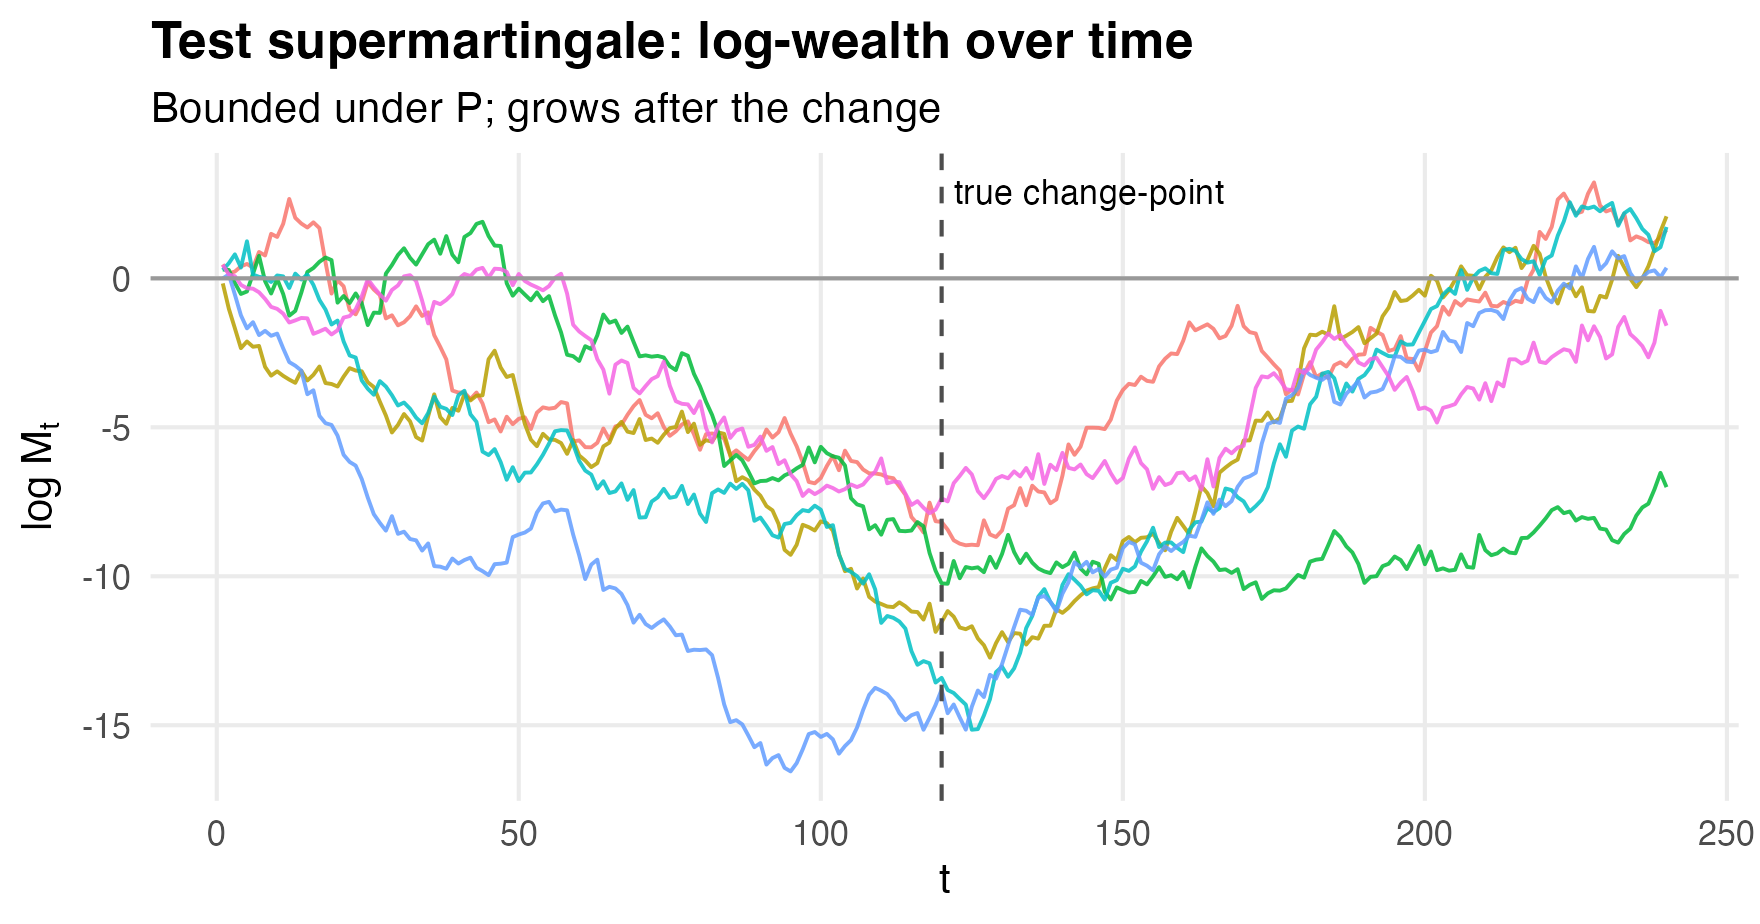
\includegraphics[width=0.6\linewidth]{figures/tsm_growth.png}\\
%   \end{center}
 
% \end{frame}

% ---------- Shiryaev-Roberts (ARL) ----------
\begin{frame}{From a TSM to a detector: Shiryaev--Roberts (\ARL\ control)}
 
  % Given a set of TSMs $(\Mt^{(i)})$ for $\mathcal{P}$, define
  % \[
  %   \boxed{\ \Rt := \sum_{i=1}^t M_t^{(i)}, \quad R_0 := 0 \ }
  %   \qquad\mbox{and}\qquad
  %   \boxed{D_{\SR} := \inf\{t : \Rt > 1/\alpha\}}.
  % \]\\
  Given a \emph{test supermartingale} $(M_t)$ for $\mathcal{P}$ with ``increments" $\Lambda_t := M_t/M_{t-1}$ define
 \[
    \boxed{\ \Rt := \Lambda_t (R_{t-1} + 1), \quad R_0 := 0 \ }
    \qquad\mbox{and}\qquad
    \boxed{D_{\SR} := \inf\{t : \Rt > 1/\alpha\}}.
  \]\\
  \vspace{3mm}
  \pause
  \textbf{Theorem:} $D_{\SR}$ is ARL-valid for $\mathcal{P}$ \citep{shiryaev_1963}\\
  \pause
  \medskip
  \vspace{3mm}
  \textbf{Statistical view:} \TSM s are (extended) likelihood ratios.\\
  \vspace{3mm}
  \textbf{Investment view:} At every step $t$, invest a fresh \$1 to start a new \TSM\
  betting against $P$ and compute $\Rt$ as the \emph{running sum} of your wealth. \\
  \medskip
  \vspace{3mm}
  \textbf{Composite pre-change}: bet against every $P \in \mathcal{P}$, $R_t$ is the smallest wealth.\\
  \vspace{3mm}
  \small
  NB: pre-estimating $P$ by $\widehat{P} \in \mathcal{P}$ is very sensitive to mis-specification \citep{mei2006sequential}

  
\end{frame}

\begin{frame}{Picture: the Shiryaev--Roberts procedure}
  \centering
  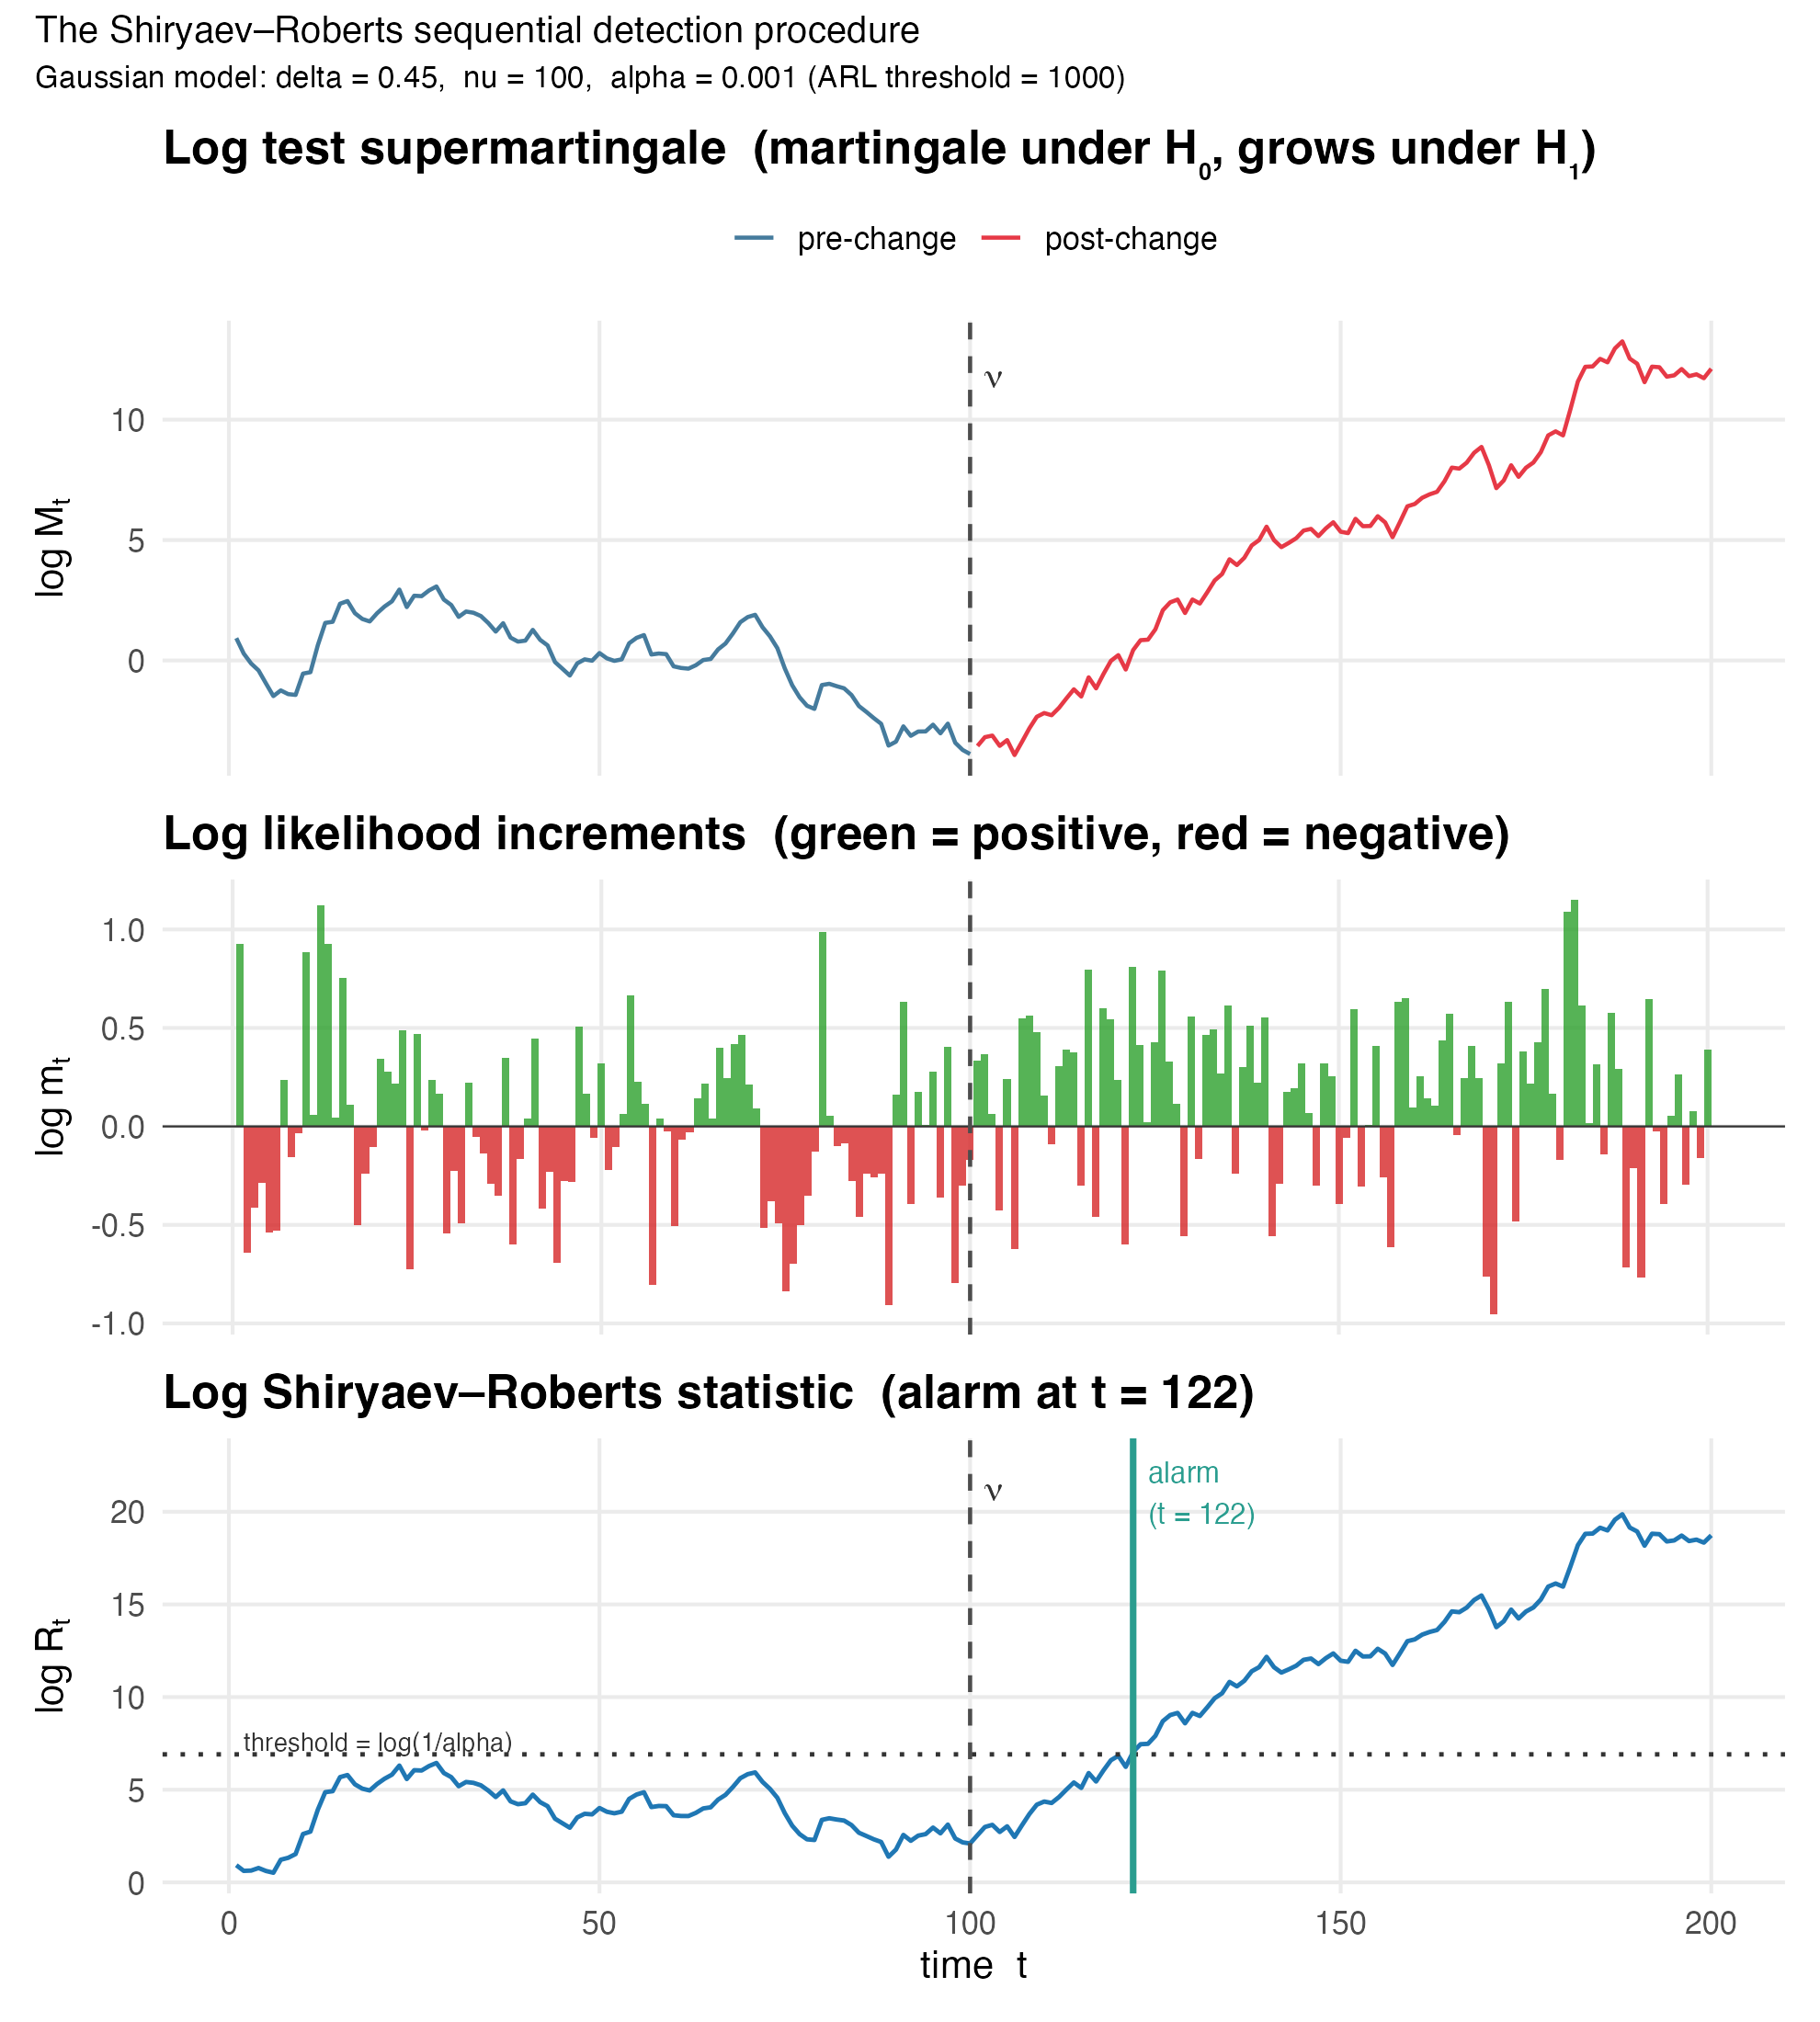
\includegraphics[width=0.5\linewidth]{figures/sr_procedure_illustration.png}\\
  \vspace{-0.5em}
\end{frame}

\begin{frame}{Nonparametric likelihood ratio TSM}
    For a non-negative data stream $(X_t)$ and predictable betting sequence $(\lambda_t)$:
    $$M_t := \prod_{i=1}^t [1 + \lambda_i (X_i - \eta_i)]$$
    is a TSM when $\mathbb{E}_P[X_t | \mathcal{F}_{t-1}] \leq \eta_t$ and $\lambda_t \in [0,1/\eta]$ for all $t$.\\
    \vspace{3mm}
    \pause
    \textbf{Features:}
    \begin{itemize}
        \item Finite-sample validity over nonparametric $\mathcal{P}$---all bounded distributions 
        \item Includes: Binomial, Beta, Poisson, truncated normal, contingency tables, finite-populations, distributions with physical constraints, within-stream dependency
    \end{itemize}
    \pause
    \textbf{Strategies:}
    \begin{itemize}
        \item Adaptive betting \citep{waudby-smithRamdas24, spertus24}
        \item Mixture betting \citep{orabona22, waudbysmith25, spertusEtal25}
        \item Handle nuisance parameters by further minimization \citep{spertus2024sequential}
    \end{itemize}
\end{frame}


\begin{frame}{Multivariate detectors}
 Let $(M_{tk})$ be any marginal \TSM\ for stream $k$, with increments $\Lambda_{tk} := M_{tk} / M_{(t-1)k}$. \\
 \vspace{3mm}
    \alert{Joint detection}: fire if \textit{any} stream changes
    \begin{itemize}
        \item \textbf{Combining:} product ($\prod_k M_{tk}$), average ($\sum_k w_k M_{tk}$), universal portfolio
        \item Product: most powerful, requires cross-stream independence \citep{vovkWang2021}
        \item Universal portfolio: larger than $\max_k M_{tk}$, computationally expensive \citep{cover1991} 
        \item Analogous to intersection testing (meta-analysis) 
    \end{itemize}
    \alert{Localized detection}: locate $K$ distinct change-points + control time to first detection
    \begin{itemize}
        \item \textbf{Spending allowance}: sum of per-time investment across streams = 1 
        \item Generalizes Bonferonni correction (threshold = $K/\alpha$)
        \item Advantages: prioritize streams, adapt to past data, employ side information, Bayesian model with frequentist validity
        \item Analogous to multiple testing (family-wise error rate) 
    \end{itemize}
\end{frame}



% \begin{frame}{Spending allowances can beat Bonferroni}
%   \textbf{Side information.}
%   If we expect change to be more likely at certain streams (priors over $k$)
%   or at certain times (priors over $t$), shift $\gamma_{tk}$ accordingly
%   \emph{predictably}.
%   \medskip

%   \textbf{Adaptivity.}
%   Once stream $k$ alarms, reallocate its remaining allowance to its neighbours
%   on a spatial graph, or to streams correlated with it.
%   \medskip

%   \textbf{Validity preserved.} Predictability of $(\gamma_t)$ is the only requirement.
% \end{frame}

% \begin{frame}{Example: graph-adaptive spending allowance}
%   \begin{columns}[T,onlytextwidth]
%     \column{0.58\textwidth}
%       \centering
%       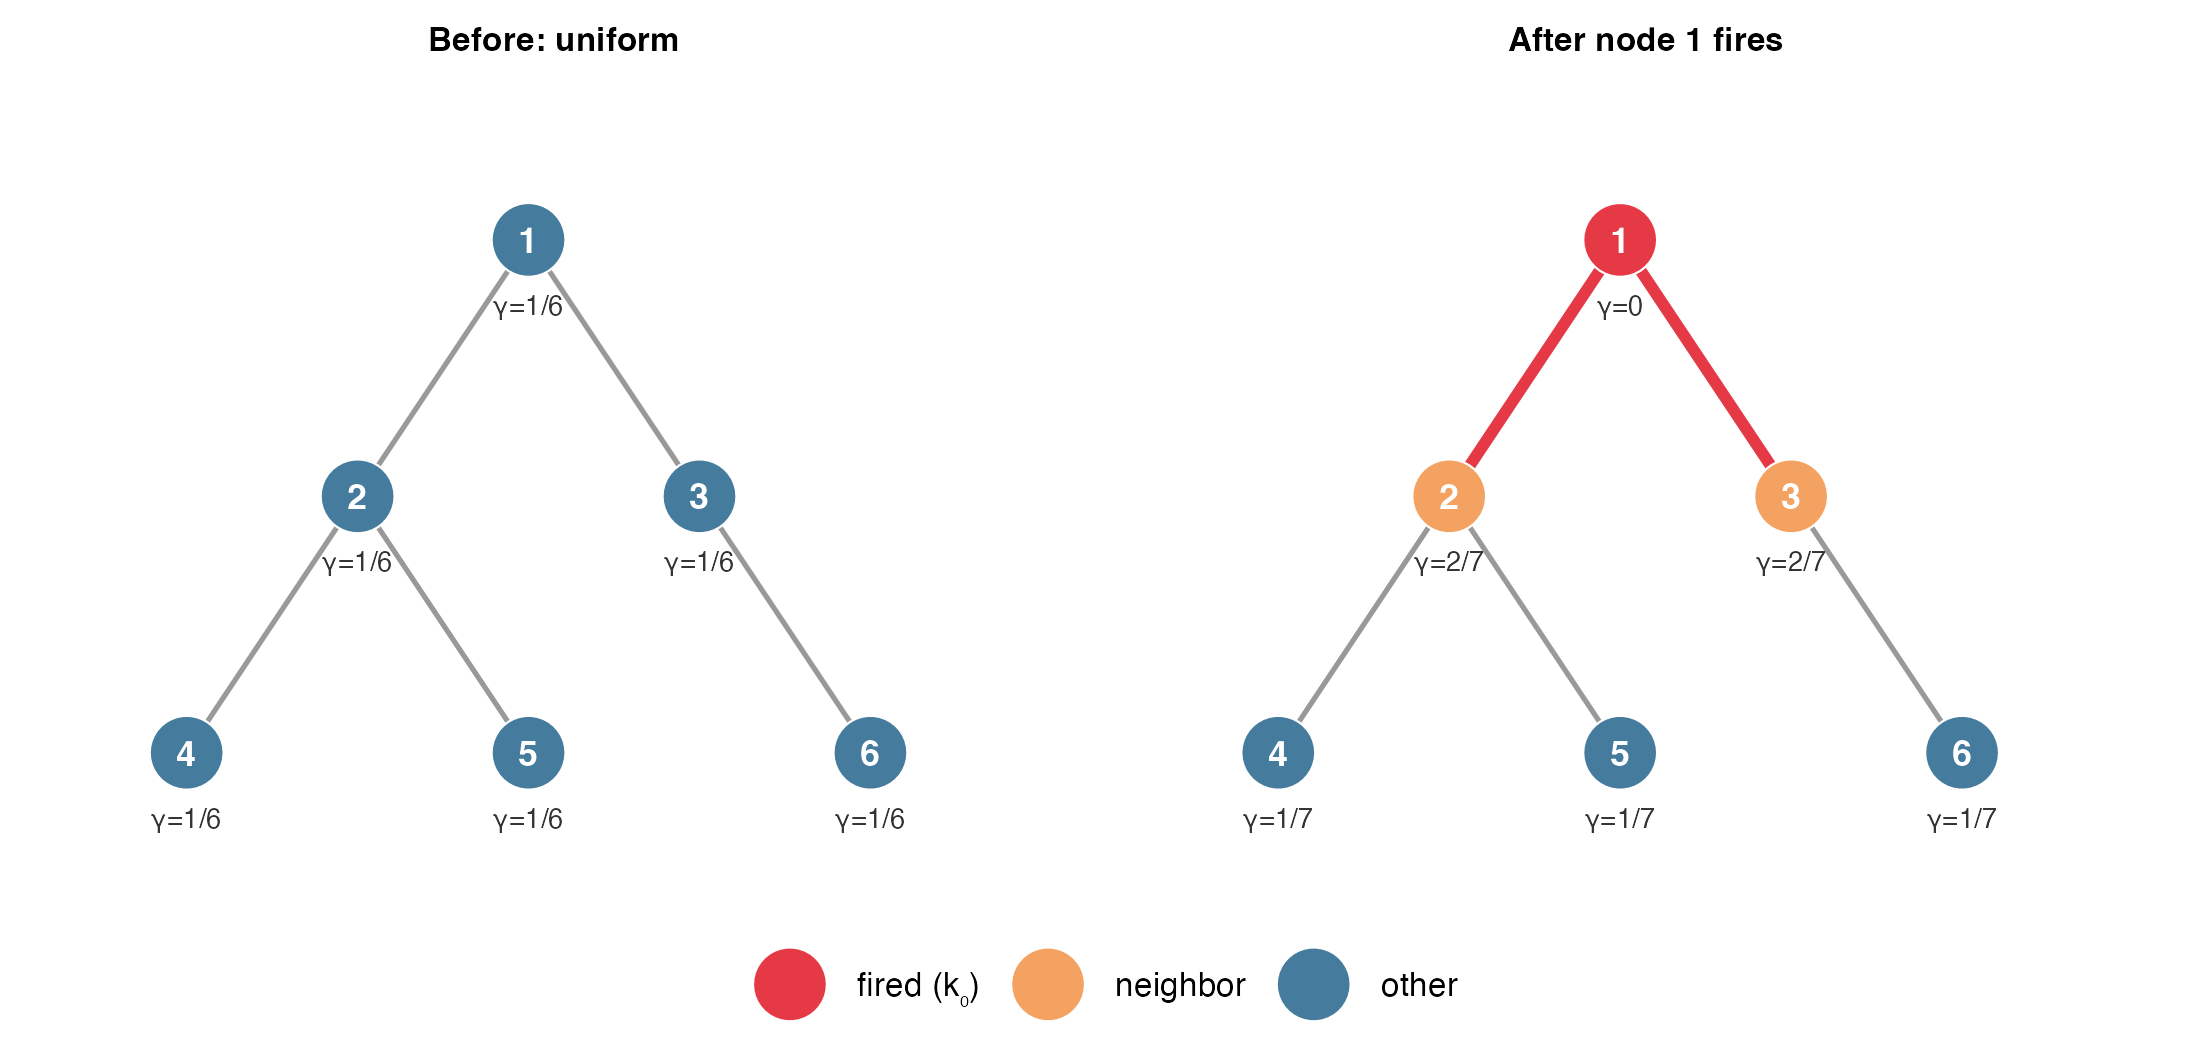
\includegraphics[width=\linewidth]{figures/graph_spending.png}
%     \column{0.42\textwidth}
%       \footnotesize
%       \textbf{Before alarm}: uniform \\
%       \medskip
%       Here: $\gamma_{tk} = \tfrac{1}{6} \quad \forall\, k$\\
%       \medskip
%       \vspace{2mm}
%       \textbf{After alarm}: refocus allowance\\
%       \medskip
%       Here:
%         $\gamma_{tk} = \Bigl(0,\;\tfrac{2}{7},\;\tfrac{2}{7},\;\tfrac{1}{7},\;\tfrac{1}{7},\;\tfrac{1}{7}\Bigr)$\\
%       \medskip
%       \vspace{3mm}
%       \textit{Any predictable allowance preserves global ARL}
%   \end{columns}
% \end{frame}

% ---------- Simulations: one key plot ----------
\begin{frame}{Simulation setup}
  
      $K$-variate Gaussian VAR model:
      $\bs{X}_t = \bs{\mu} + \sum_{j=1}^p \bs{\Phi}_j (\bs{X}_{t-j} - \bs{\mu}) + \bs{\varepsilon}_t ~~\mbox{with}~~ \bs{\varepsilon}_t \sim \mathcal{N}(\bs{0}, \bs{\Sigma})$
  \begin{itemize}
  \item $\mathcal{P}$: $\bs{\mu}_0 := 0.3 \times \bs{1}$, $\bs{\Phi} = \bs{0}$, $\bs{\Sigma} = \mbox{diag}(0.05^2)$ 
  \item $\mathcal{Q}$: $\bs{\mu}_1 := \bs{\mu}_0 + {\bs{1}} \times \delta / \sqrt{K}$ (\textit{dense change}) or  $\bs{\mu}_1 := \bs{\mu}_0 +  {\bs{e}_1} \times \delta$ (\textit{sparse change})
  \item Four detectors:
  \begin{itemize}
      \item Oracle TSM (true Gaussian VAR)
      \item Bounded TSM + adaptive bets + product combining 
      \item Bounded TSM + adaptive bets + average combining
      \item Mis-specified Gaussian VAR TSM (plug-in $\bs{\mu}_1 + 0.2 \times \bs{1})$
  \end{itemize}
  \item Model extensions: streams $K$, coefficients $\Phi$, covariance $\bs{\Sigma}$, order $p$, DGP
  \item Detector extensions: universal portfolio combining, localization with spending allowances, PFA control with spending schedule
  \end{itemize}
\end{frame}


\begin{frame}{Optimal CAD and regret in Gaussian VAR}
  \centering
  
\includegraphics[width=0.7\linewidth]{figures/joint_oracle_vs_bounded.png}\\
\end{frame}

% ============================================================
\section{Part 2 --- Wastewater surveillance}
% ============================================================

\begin{frame}{Wastewater monitoring as a multi-stream change-point problem}
  \textbf{Setting.}
  Canadian \textsc{nwmp}: a graph of wastewater treatment sites,
  each producing weekly viral signal time series for COVID, RSV, influenza, $\ldots$\\
  \vspace{5mm}
  \medskip
    
  \textbf{Public-health use case.}
  Past work (Peng et al., Ottawa) links viral signals to leading clinical
  indicators (hospitalizations 1--3 weeks out). Detection $\Rightarrow$
  flag sites and triage resources.\\
  \vspace{5mm}
  \medskip
  % \textbf{Challenges:}
  % population state-of-control is uncertain, noise in population + sampling, composite null/alternative, multiple streams, multiple change-points, premium on simplicity
\end{frame}

\begin{frame}{Sources of noise and systematic uncertainty}
  \begin{itemize}\setlength\itemsep{0.3em}
    \item \textbf{Catchment.} Boundaries differ across sites; may not align with clinical catchment areas.
    \vspace{3mm}
    \item \textbf{Water volume.} Open vs.\ closed sewage systems; weather events.
    \vspace{3mm}
    \item \textbf{Sampling design.} Auto vs.\ grab; compositing; lab protocols.
    \vspace{3mm}
    \item \textbf{Demography.} Secular and seasonal shifts in resident population.
    \vspace{3mm}
    \item \textbf{Endemicity.} Even ``baseline'' COVID has a seasonal contour.
  \end{itemize}
\end{frame}

\begin{frame}{What is the ``state of control''?}
  Even with perfect data, the target is ambiguous. A working definition:
  \medskip

   \textbf{Operational state of control:} 
    Covid signal moves \emph{in line with} a reference virus
    (RSV, pMMoV) and with the historical seasonal contour observed in
    2023--2025.
  \medskip

  \textbf{Concretely:} Normalize weekly covid signal by reference virus, de-seasonalize,
  and treat residuals as the monitored stream. Detection fires when covid is
  \emph{unseasonably high} relative to its long-run movement with the
  reference.
  \medskip

  \alert{Caveat}:
  Different stakeholders may consider different states of control important
  (e.g.\ absolute thresholds, residual correlation with leading hospitalizations).
\end{frame}

\begin{frame}{Pipeline}
  \centering
  \resizebox{\textwidth}{!}{
  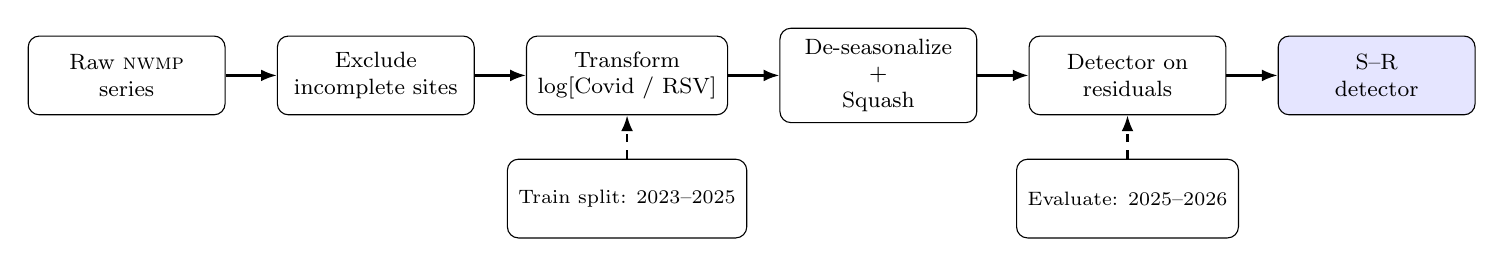
\begin{tikzpicture}[
      node distance=0.55cm and 0.65cm,
      box/.style={draw, rounded corners, align=center, font=\footnotesize,
                  inner sep=4pt, minimum height=1.0cm, minimum width=2.5cm},
      arr/.style={-{Latex[length=2mm]}, thick}
    ]
    \node[box] (raw)   {Raw \textsc{nwmp} \\ series};
     \node[box, right=of raw] (exc) {Exclude \\ incomplete sites};
    \node[box, right=of exc] (trans) {Transform \\ $\log [\mbox{Covid / RSV}]$};
    \node[box, right=of trans] (des)  {De-seasonalize \\ + \\ Squash};
    \node[box, right=of des] (var)  {Detector on\\residuals};
    \node[box, right=of var, fill=blue!10] (det) {S--R \\ detector};
    \draw[arr] (raw) -- (exc);
    \draw[arr] (exc) -- (trans);
    \draw[arr] (trans) -- (des);
    \draw[arr] (des) -- (var);
    \draw[arr] (var) -- (det);

    \node[box, below=of trans, font=\scriptsize] (split1) {Train split: 2023--2025};
    \node[box, below=of var, font=\scriptsize] (split2) {Evaluate: 2025--2026};
    \draw[arr, dashed] (split1) -- (trans.south);
    \draw[arr, dashed] (split2) -- (var.south);
  \end{tikzpicture}
  }
  \medskip
  \scriptsize Pre-change parameters are learned on the held-out 2023--2025
  window; the detector is run forward on 2025--2026 with no further refitting.

  
\end{frame}

\begin{frame}{Empirical: detector trajectory on 2025--2026 season}
  \begin{columns}[T,onlytextwidth]
      \column{0.5\textwidth}
      
\includegraphics[width = 0.9\linewidth]{figures/pipeline-plot-2.png}\\
      \scriptsize
       $\log \Rt$ vs.\ time with threshold $\log(1/\alpha)$ for $\alpha = 1/(52*5)$.\\
       \column{0.5\textwidth}
       Montreal alarms in October \\
       \vspace{3mm}
       Charlottestown + Stratford in December\\
       \vspace{3mm}
       Generally, detectors fire when ratios are \emph{sustained} above training period levels\\
       \vspace{3mm}
       Faster detection by pre-specifying post-change distribution(s)
   \end{columns}
\end{frame}

\begin{frame}{Simple approach: threshold signals}
    \begin{columns}[T,onlytextwidth]
      \column{0.5\textwidth}
      
\includegraphics[width=0.9\linewidth]{figures/threshold-baseline-test-1.png}\\
      \scriptsize
       Alarm times with simple threshold rule\\
       \column{0.5\textwidth}
       Take some (e.g. 95th) percentile of raw COVID signals on 2023-2025 data\\
       \vspace{3mm}
       Alarm if percentile threshold is exceeded going forward\\
       \vspace{3mm}
       Edmonton alarms in July, Montreal and Toronto in February, St John's in September\\
       \vspace{3mm}
       Simple and transparent\\
       \vspace{3mm}
       Statistical properties are unknown...\\
       \vspace{3mm}
       But DGP is unknown, so this is true anyway
   \end{columns}
\end{frame}

% \begin{frame}{Localization on the WW site graph}
%   \textbf{Idea.} Treat sites as a graph (spatial adjacency, catchment overlap,
%   shared-platform clusters). Run per-site detectors with a \emph{spending
%   allowance} that:
%   \begin{itemize}
%     \item gives equal $\gamma_{tk}$ pre-firing (Bonferroni-equivalent), and
%     \item after firing at site $k^\star$, reallocates $k^\star$'s remaining
%       allowance to its neighbours via a Bayesian posterior over spread.
%   \end{itemize}
%   \medskip
%   \centering
%   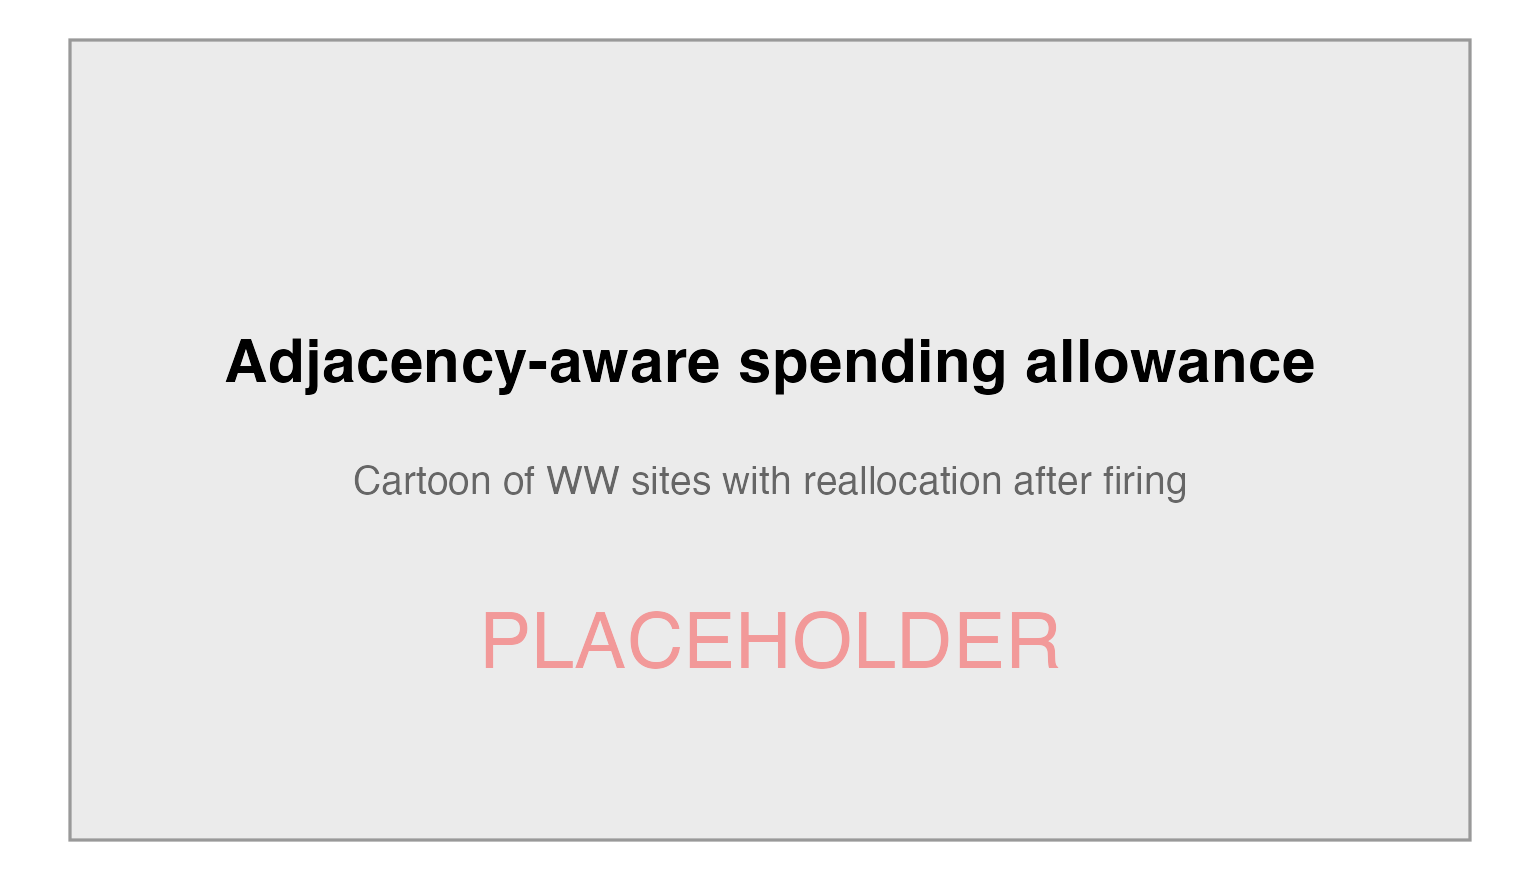
\includegraphics[width=0.55\linewidth]{figures/ww_localization_placeholder.png}\\
%   \scriptsize Placeholder: adjacency-aware allocation cartoon.
% \end{frame}

% ============================================================
\section{Wrap-up}
% ============================================================

\begin{frame}{Summary}
  \begin{itemize}\setlength\itemsep{0.4em}
    \item Detectors are bets. Validity follows from the \TSM\ + Ville's inequality.
    \item Shiryaev--Roberts $\Rightarrow$ \ARL\ control.
    \item Multivariate combining is meta-analysis: product / average / universal portfolio.
    \item Localization is multiple testing with a predictable spending allowance.
    \item Wastewater: composite pre-change, dependent streams,
      multiple sites, drift.
  \end{itemize}
  \medskip

  \textbf{What else:}
  PFA control with spending schedule; efficient computation; incorporating clinical signals in WWM; extending to additional sites.
\end{frame}

\begin{frame}[standout]
  Thank you.\\[0.6em]
  {\normalsize \texttt{jakespertus@gmail.com}} \\
  {\normalsize \texttt{https://github.com/spertus/multivariate-change-point-detection/}}
\end{frame}

\begin{frame}{References}
\tiny 
    \bibliographystyle{apalike}
    \bibliography{cpd_bib.bib}
\end{frame}

% ============================================================
\appendix




\begin{frame}{Appendix: bounded model and \textsc{AGRAPA} bets}
  \textbf{Model assumptions:} $\X_t \in [0,1]^K$, $\E_P[X_{tk} \mid \Fc_{t-1}] \le \eta_k$ .
  \medskip

  \textbf{Marginal betting \TSM.}
  \[
    M^k_t = \prod_{i =1}^t \bigl[1 + \lambda_{ik}(X_{ik} - \eta_k)\bigr],\qquad
    \lambda_{ik} \in [0, 1/\eta_k]\ \text{predictable}.
  \]

  \textbf{\textsc{AGRAPA} \citep{waudby-smithRamdas24}}
  \[
    \lambda_{tk} = 0 \vee
    \frac{2(\hat\mu_{k(t-1)} - \eta_k)}{\hat\sigma_{k(t-1)}^2 + (\hat\mu_{k(t-1)} - \eta_k)^2}
    \wedge \frac{c}{\eta_k}.
  \]
\end{frame}

\begin{frame}{Appendix: CAD for bet windowing strategies over $\nu$}
    \centering
    
\includegraphics[width = \textwidth]{figures/bounded_nu_cad.png}\\
    \scriptsize
    Conditional average delay of bounded TSMs + S-R procedure using different AGRAPA strategies
\end{frame}

\begin{frame}{Appendix: Computation time for bet windowing strategies}
    \centering
    
\includegraphics[width = \textwidth]{figures/bounded_w_comp_time.png}\\
    \scriptsize
    Computation time for bounded TSMs + S-R procedure using different AGRAPA strategies
\end{frame}

% ---------- Multivariate combining ----------
\begin{frame}{Appendix: joint detectors via meta-analysis of TSMs}
  \alert{Goal}: detector fires if \emph{any} stream changes \\ 
  \medskip
  Let $(M_{tk})$ be any marginal \TSM\ for stream $k$, with increments $\Lambda_{tk} := M_{tk} / M_{(t-1)k}$.
  \medskip
  \begin{block}{Three ways to combine:}
    \begin{description}[align = left]
      \item[\textbf{Product}] $M_t^p = \prod_k M_{tk}$ \hfill (valid \emph{iff} streams are independent)
      \item[\textbf{Average}] $M_t^a = \sum_k w_k M_{tk}$ with $\sum w_k = 1$  \hfill (valid under \emph{arbitrary} dependence)
      \item[~~~~\textbf{Universal portfolio}] $M_t^u = \int_{\mathcal{S}^K} \prod_{i=1}^t \sum_{k=1}^K u_k \Lambda_{ik}\,d{\bs{u}}$ \hfill (always valid, better than average)
      % \item[~~~~\textbf{Maximum}] $M_t^m = \max_k M_{tk}$ \hfill (never valid!)
    \end{description}
  \end{block}
  \medskip
  Asymptotically, $M_t^u \geq \max_k M_{tk}$ \citep{cover1991}, but $M_t^u$ is hard to compute\\
  \medskip
  \textbf{Analogue:} intersection testing (meta-analysis) with $E$-values \citep{vovkWang2021}
  \medskip
\end{frame}


% \begin{frame}{Combiners on the same data}
%   \centering
%   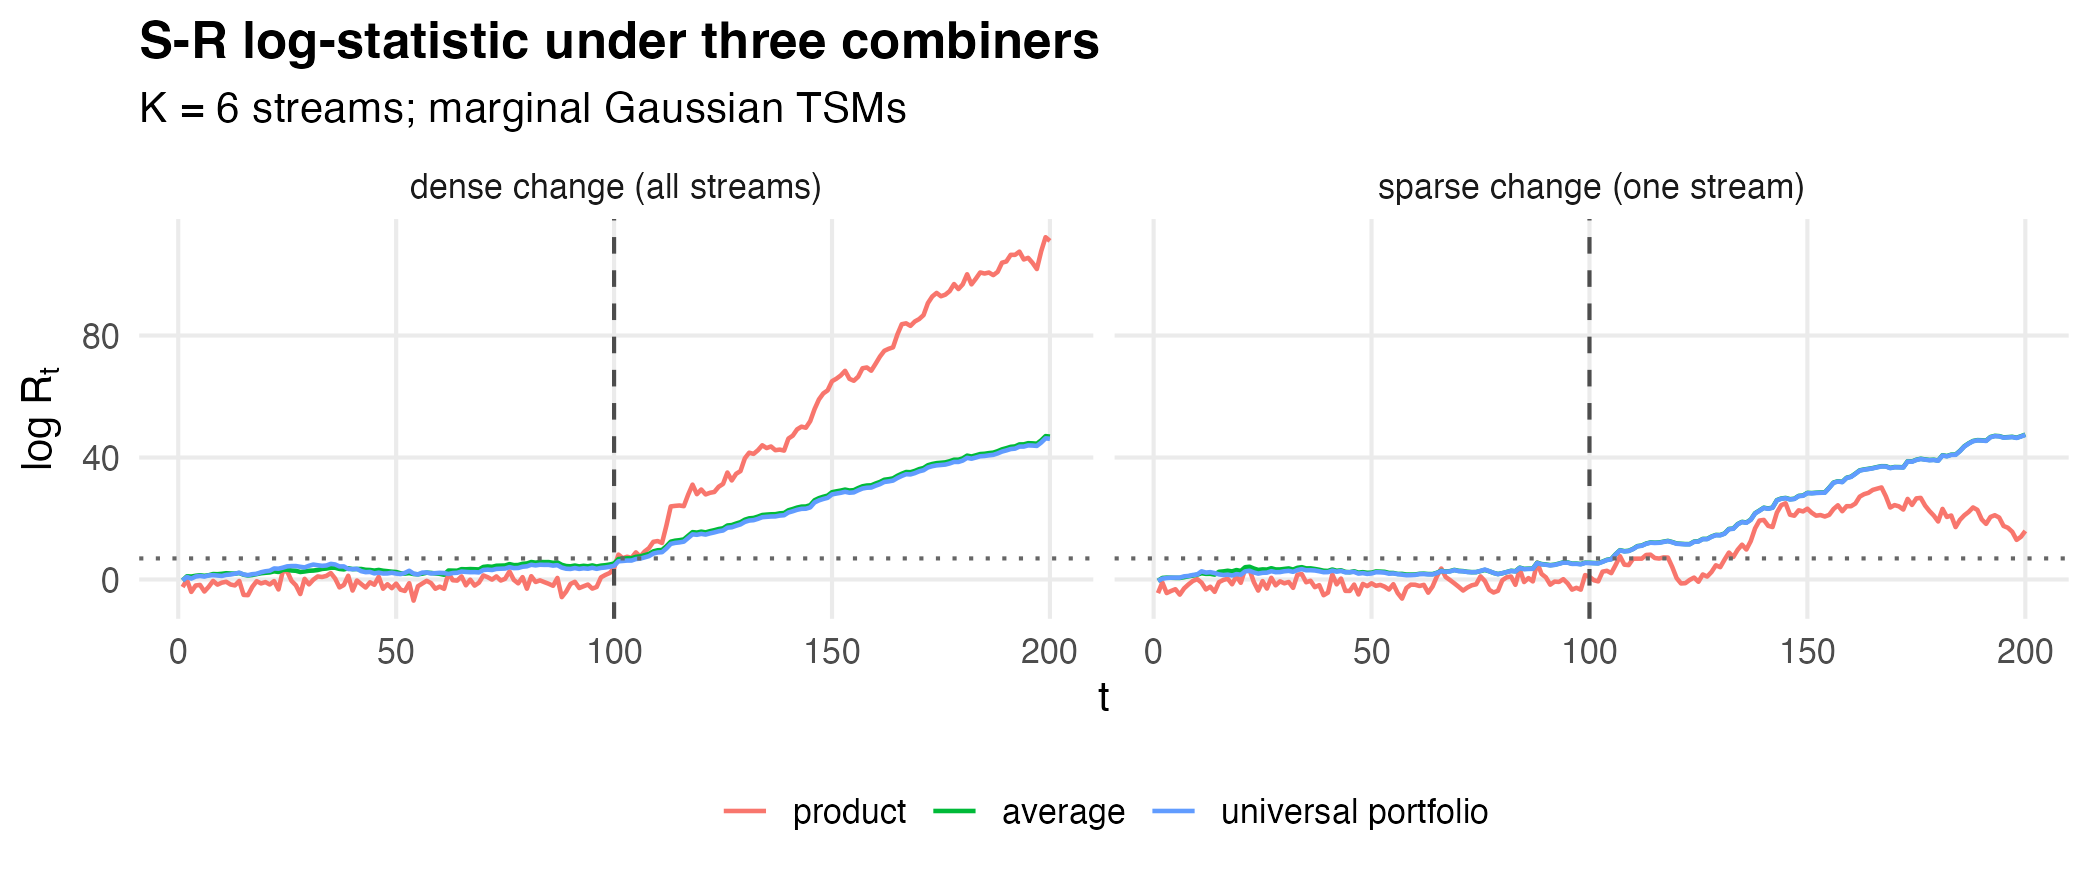
\includegraphics[width=0.95\linewidth]{figures/combiners_paths.png}\\
%   \scriptsize Same realizations as above, $K=6$, $\alpha = 10^{-3}$.
%   Under sparse change UP $\approx$ product; under dense change product compounds fastest.
% \end{frame}

% ---------- Localization ----------
\begin{frame}{Appendix: localization}
 \alert{Goal}: $K$ change points $\{\nu_k\}_{k=1}^K$ $\implies$ $K$ detectors  \\ 
    \medskip
   Require $\bm{D} = [D_1, \ldots, D_K]$ to control the \emph{global} \ARL:
  \[
    \ARL(\bm{D}) := \sup_{P}\E_{P,\infty}\!\left[\min_k D_k\right]
  \]
  \medskip
  \textbf{Testing analogue:} multiple testing / family-wise error rate. \\
  \medskip 
   \textbf{Union bound:} set each detector's threshold to $K/\alpha$\\
   \medskip
   This is the Bonferonni correction, which is crude...
\end{frame}

\begin{frame}{Appendix: spending allowance}
    A \alert{spending allowance} $(\gamma_t)$ has $\sum_k \gamma_{tk} = 1$ at \emph{each} time.\\
    \medskip
    \textbf{Theorem:} Thresholding each $R_{tk}^\gamma := \Lambda_{tk} (R_{(t-1)k}^\gamma + \gamma_{tk})$ controls the global ARL \\
    \medskip
    $(\gamma_t)$ may be predictable, adapting to past data + side information\\
    \medskip
    Examples:
    \begin{itemize}
        \item $\gamma_{tk} := 1/K \implies$ Bonferonni
        \item Weighted $\gamma_{tk}$ $\implies$ prioritize more important streams 
        \item Bayesian posterior on $\gamma_{tk}$ $\implies$ model on alarms
        \item Graph-adaptive $\gamma_{tk}$ $\implies$ nearby sites more likely to alarm together (clusters)
    \end{itemize}
\end{frame}


\begin{frame}{Appendix: full \ARL\ theorem}
  \begin{block}{Theorem (S--R is \ARL-valid).}
    Given any \TSM\ $(\Mt)$ under $\Pc$ with increments $\Lt = \Mt/M_{t-1}$,
    \(\Rt := \Lt(R_{t-1} + 1)\) yields
    \(D_{\SR} := \inf\{t : \Rt > 1/\alpha\}\) with
    \(\sup_{P\in\Pc} \E_{P,\infty}[D_{\SR}] \ge 1/\alpha.\)
  \end{block}
  \medskip
  \textbf{Sketch.} $\Rt - t$ is a $P$-supermartingale; apply Doob's optional stopping
  theorem at $D_{\SR}$ and use $R_{D_{\SR}} \ge 1/\alpha$.
\end{frame}

\begin{frame}{Appendix: full \PFA\ theorem}
  \begin{block}{Theorem (scheduled S--R is \PFA-valid).}
    With spending schedule $(\pi_t)$, $\sum_t \pi_t = 1$, and
    \(\Rt^\pi := \Lt(R_{t-1}^\pi + \pi_t),\) the detector
    \(D^\pi := \inf\{t : \Rt^\pi > 1/\alpha\}\) satisfies
    \(\sup_{P\in\Pc}\Prob_{P,\infty}(D^\pi < \infty) \le \alpha.\)
  \end{block}
  \medskip
  \textbf{Sketch.} Telescoping gives $\Rt^\pi = \sum_i \pi_i M_t^{(i)}$,
  a convex combination of delayed \TSM s---hence itself a \TSM. Apply Ville.
\end{frame}



\begin{frame}{Appendix: Gaussian VAR($p$) increment}
  \[
    \log \Lt = \tfrac{1}{2}\log\frac{|\Sigma_0|}{|\Sigma_1|}
    + \tfrac{1}{2}\Bigl[ (\Xt - m_t^0)^\top \Sigma_0^{-1}(\Xt - m_t^0)
      - (\Xt - m_t^1)^\top \Sigma_1^{-1}(\Xt - m_t^1) \Bigr]
  \]
  where $m_t^i = \mu_i + \sum_{j=1}^p \Phi_j^{(i)} (\X_{t-j} - \mu_i)$.
  \medskip

  Coordinate-free expression: change in $\mu$, $\Phi_j$, or $\Sigma$ shows up
  through the displacement of conditional means $m_t^1 - m_t^0$.
\end{frame}

% ---------- Spending schedule (PFA) ----------
\begin{frame}{Spending schedules: trading \ARL\ control for \PFA\ control}
  A \alert{spending schedule} $(\pi_t)$ is a pmf on $\N$: $\sum_t \pi_t = 1$.
  Run a \emph{scheduled} S--R:
  \[
    \boxed{\ \Rt^\pi := \Lt \cdot (R_{t-1}^\pi + \pi_t) \ }
    \qquad
    D^\pi := \inf\{t : \Rt^\pi > 1/\alpha\}.
  \]
  \pause
  \textbf{Theorem (this work).} $\Prob_{P,\infty}(D^\pi < \infty) \le \alpha$.
  \medskip

  \textbf{Investment view.} Instead of a fresh \$1 each step,
  spend only $\pi_t$ at time $t$; total lifetime budget capped at \$1.
  \medskip

  $(\pi_t)$ is \emph{like} a prior on $\nu$, but validity does \emph{not} depend on
  the prior being correct---only efficiency does.
\end{frame}

\begin{frame}{Picture: spending schedules and their detectors}
  \centering
  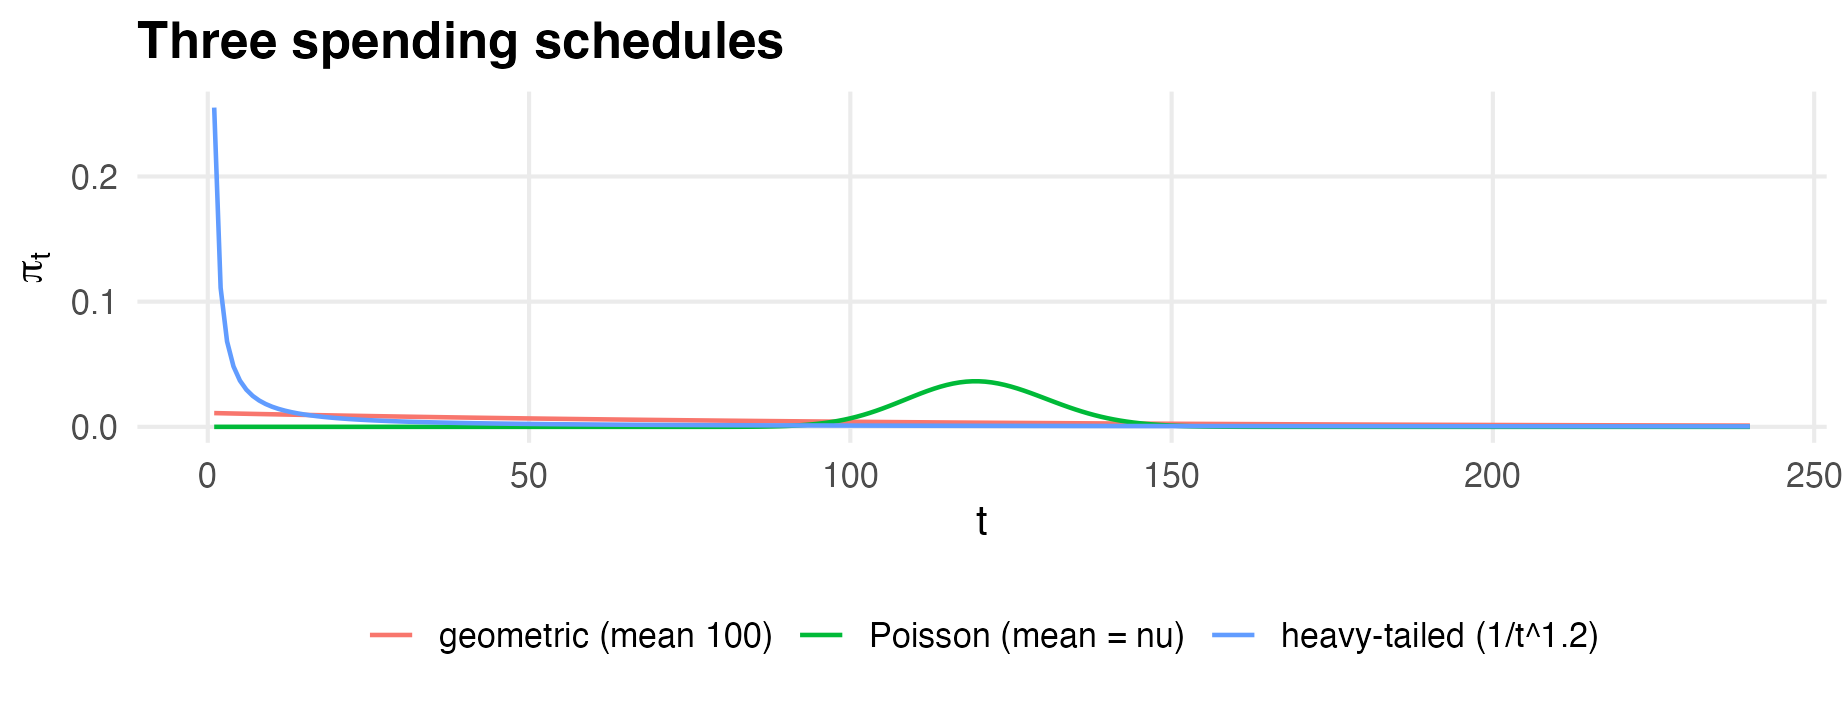
\includegraphics[width=0.65\linewidth]{figures/spending_schedule.png}\\[0.2em]
  \centering
  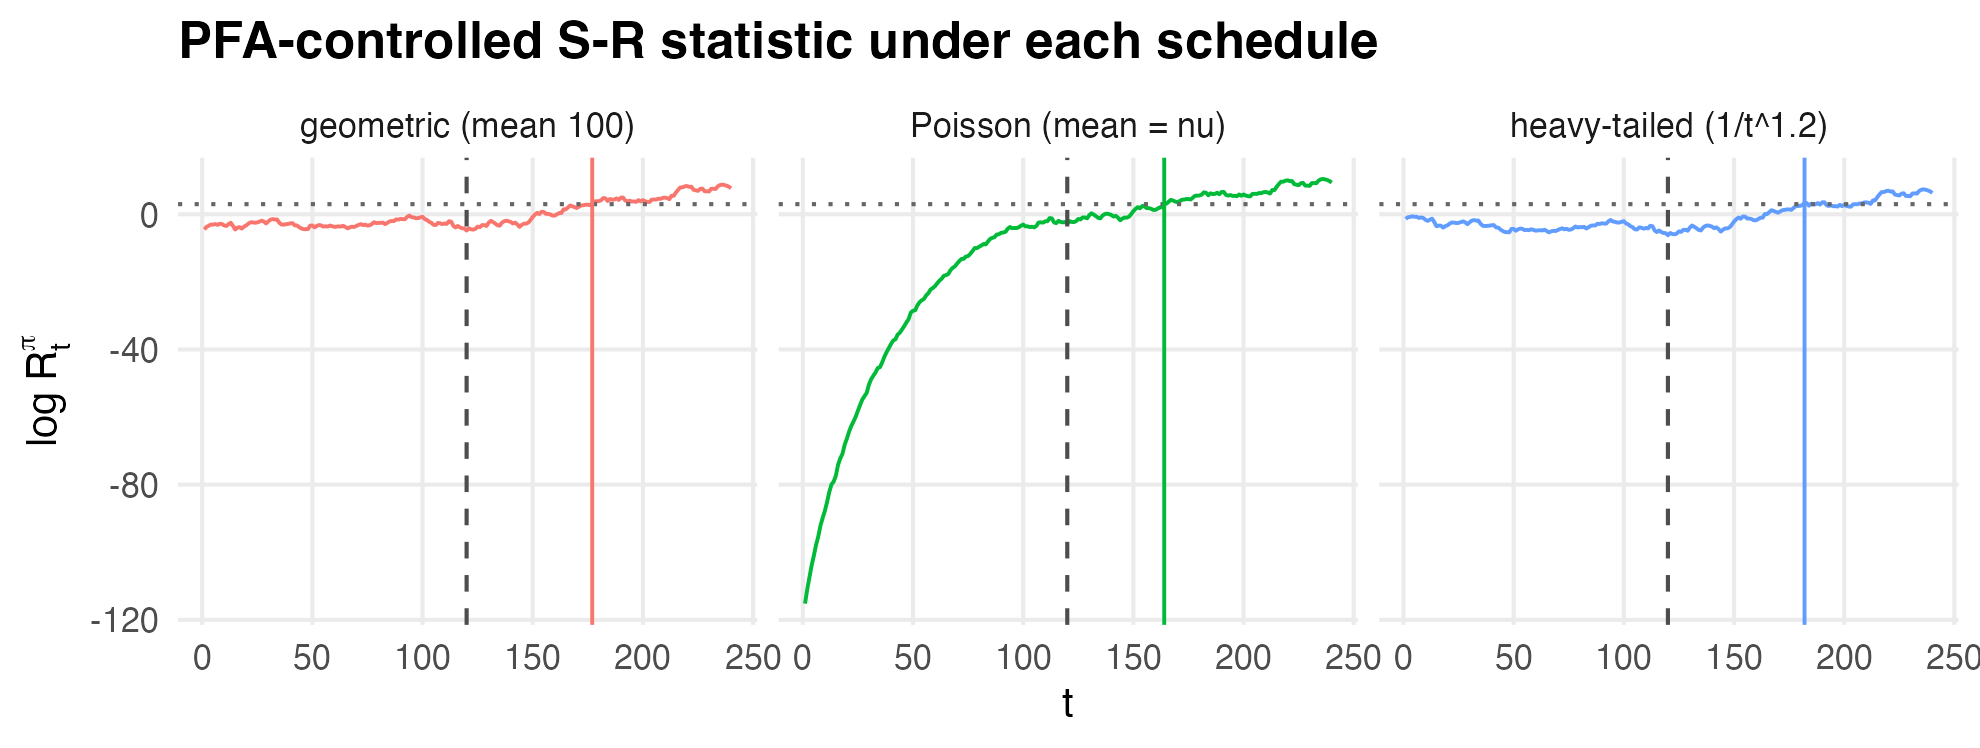
\includegraphics[width=0.65\linewidth]{figures/spending_schedule_detectors.png}\\
  \vspace{-0.4em}
  \scriptsize Spending schedules and \PFA-controlled \SR\ statistic
  under each. Concentrated schedules are efficient when $\nu$ sits in their bulk; wider schedules hedge over a range of $\nu$.
\end{frame}

% \begin{frame}{\ARL\ vs.\ \PFA: what does the cost look like?}
%   \begin{columns}[T,onlytextwidth]
%     \column{0.5\textwidth}
%       \textbf{\ARL-control.}
%       \begin{itemize}
%         \item Renew \$1 every step.
%         \item Detector restarts after each false alarm.
%         \item Cheap delay; many false alarms over an infinite horizon.
%       \end{itemize}
%     \column{0.5\textwidth}
%       \textbf{\PFA-control.}
%       \begin{itemize}
%         \item Total budget \$1.
%         \item No false alarms ever (w.p.\ $1-\alpha$).
%         \item Pays in efficiency unless $\pi$ concentrates near $\nu$.
%       \end{itemize}
%   \end{columns}
%   \medskip
%   \centering
%   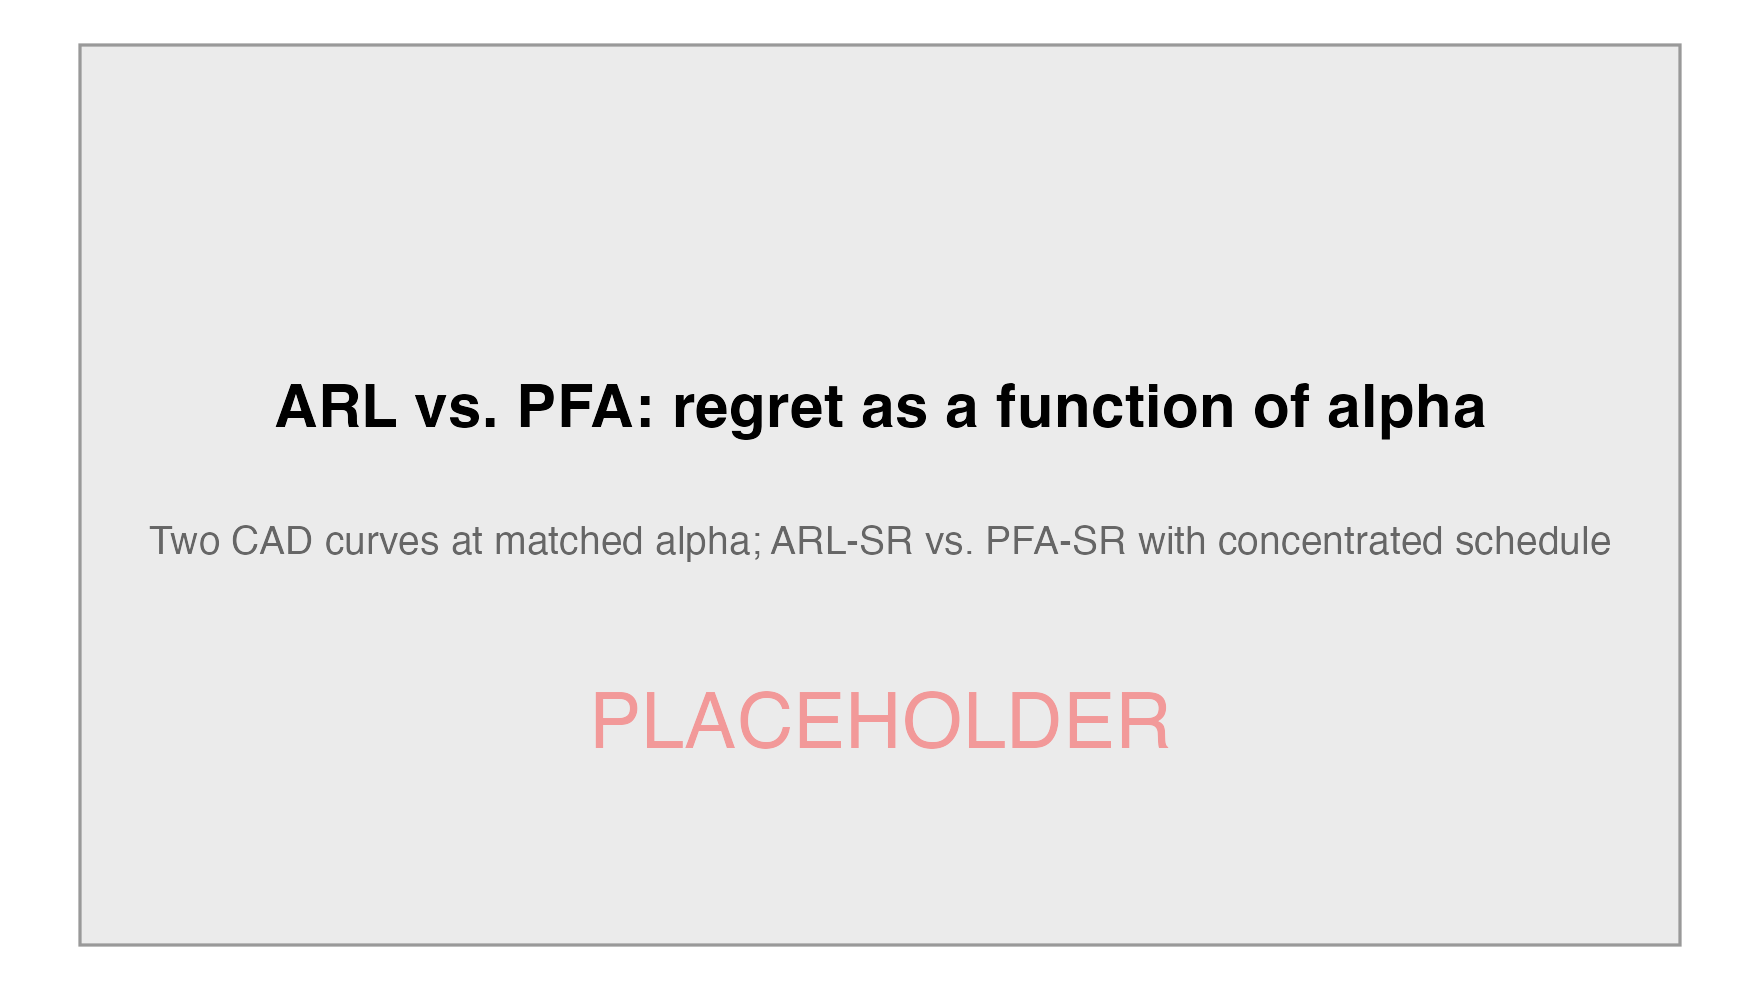
\includegraphics[width=0.65\linewidth]{figures/arl_vs_pfa_placeholder.png}
% \end{frame}

% ---------- Composite alternative (one slide, light) ----------
% \begin{frame}{Composite alternatives: three valid options}
%   When $\Qc$ is composite, the increment $\Lt$ needs a value for $\theta$.
%   \medskip
%   \begin{enumerate}\setlength\itemsep{0.4em}
%     \item \textbf{Mixture \TSM.} Place a prior $\pi(\theta)$ on $\Omega_1$ and integrate.
%     \[
%       L_t^{\mathrm{mix}} = \int_{\Omega_1} \prod_{i\le t} \frac{f_\theta(X_i \mid \Hc_i)}{f_{\hat\theta_0^t}(X_i \mid \Hc_i)}\,\pi(\theta)\,d\theta
%     \]
%     \item \textbf{Predictable plug-in.} Pick any $\hat\theta_{i-1}$ measurable in $\Hc_{i-1}$
%       (online MLE, posterior mean, ML model, $\ldots$).
%     \item \textbf{Online learning bets.} For bounded means, \textsc{agrapa}-style bets
%       based on lagged sample mean and variance.
%   \end{enumerate}
%   \medskip
%   \alert{All three preserve the \TSM\ property, hence validity.}
% \end{frame}



\end{document}
